\documentclass[a4paper]{report}
\usepackage[group-separator={,},group-minimum-digits={3}]{siunitx}
\usepackage[utf8]{inputenc}
\usepackage[dvipsnames]{xcolor}
\usepackage{soul}
\usepackage{tcolorbox}
\usepackage{multicol}
\usepackage{lipsum}
\usepackage[margin=0.2in]{geometry}
\usepackage{xstring}
\usepackage{xifthen}
\usepackage[dvipsnames]{xcolor}
\usepackage{setspace}
\usepackage{amsmath}
\usepackage{enumitem}
\pagenumbering{gobble}
\setlength{\columnsep}{1.5cm}
\setlength{\columnseprule}{0.2pt}
\usepackage{hyperref}
\usepackage[none]{hyphenat}
\usepackage{graphicx}
\usepackage{etoolbox}
\usepackage{titlepic}
\usepackage[super]{nth}
\usepackage{setspace}
\usepackage[document]{ragged2e}

\hypersetup{
    colorlinks,
    citecolor=black,
    filecolor=black,
    linkcolor=black,
    urlcolor=black
}

\usepackage[default]{sourcesanspro}
\usepackage[T1]{fontenc}

\makeatletter
\def\@makechapterhead#1{%
  %\vspace*{5\p@}%
  {\parindent \z@ \raggedleft \normalfont
    \ifnum \c@secnumdepth >\m@ne
        \large\bfseries #1
        \par\nobreak
%        \vskip 10\p@
        \rule{\columnwidth}{.1pt}%
%        \vskip 10\p@
    \fi
    \interlinepenalty\@M
%    \large \bfseries \MakeUppercase{#1}\par\nobreak
%    \vskip 5\p@
  }}
\makeatother

\makeatletter
 \def\SOUL@hlpreamble{%
 \setul{}{3ex}%         !!!change this value!!! default is 2.5ex
 \let\SOUL@stcolor\SOUL@hlcolor
 \SOUL@stpreamble
 }
\makeatother

\newcommand{\important}[1]{\textbf{\textcolor{Red}{\hl{#1}}}}

\newcommand{\blitzloss}{\textbf{\textcolor{Magenta}{Blitz Loss}}}
\newcommand{\lostblitz}{\textbf{\textcolor{Magenta}{lost Blitz}}}

\newcommand{\blitzwin}{\textbf{\textcolor{OliveGreen}{Blitz Win}}}
\newcommand{\wonblitz}{\textbf{\textcolor{OliveGreen}{won Blitz}}}

\newcommand{\category}{FFX - No Sphere Grid (with Flee)}

\usepackage{enumitem}
\setitemize{noitemsep,topsep=0pt,parsep=0pt,partopsep=0pt}
\usepackage{graphicx}
\ifthenelse{%
		\equal{\blitzresult}{win}
	}{%
		\title{\category - \blitzwin}
	}{%
		\ifthenelse{%
			\equal{\blitzresult}{loss}
		}{%
			\title{\category - \blitzloss}
		}{%
			\ifthenelse{%
				\equal{\blitzresult}{both}
			}{
				\title{\category}
			}{}
		}
	}
\author{CrimsonInferno9}
\titlepic{
\includegraphics[width=\textwidth]{final_fantasy_x_logo_by_eldi13_d4204zv}}
\begin{document}
\singlespacing
\maketitle
\tableofcontents

\makeatletter
\patchcmd{\chapter}{\if@openright\cleardoublepage\else\clearpage\fi}{}{}{}
\makeatother

\newenvironment{battle}[2][]{\begin{tcolorbox}[title=\begin{center}\MakeUppercase{#2} \ifthenelse{\isempty{#1}}{}{- \num{#1} HP}\end{center},colbacktitle=red!50!white,colframe=red!55,coltitle=black]}{\end{tcolorbox}}

\newenvironment{shop}[1]{\begin{tcolorbox}[title=\begin{center}SHOP\, #1 GIL\end{center},colbacktitle=blue!50!white,coltitle=black,colframe=blue!50!white]}{\end{tcolorbox}}

\newenvironment{spheregrid}{\begin{tcolorbox}[title=\begin{center}SPHERE GRID\end{center},colbacktitle=purple!50!white,colframe=purple!55,coltitle=black]}{\end{tcolorbox}}

\newenvironment{encounters}{\begin{tcolorbox}[title=\begin{center}ENCOUNTERS\end{center},colbacktitle=VioletRed!50!white,colframe=VioletRed!55,coltitle=black]}{\end{tcolorbox}}

\newenvironment{trial}{\begin{tcolorbox}[title=\begin{center}CLOISTER OF TRIALS\end{center},colbacktitle=Bittersweet!50!white,colframe=Bittersweet!55,coltitle=black]}{\end{tcolorbox}}

\newenvironment{blitzball}{\begin{tcolorbox}[title=\begin{center}BLITZBALL\end{center},colbacktitle=Maroon!50!white,coltitle=black,colframe=Maroon!50!white]}{\end{tcolorbox}}

\newenvironment{equip}{\begin{tcolorbox}[title=\begin{center}EQUIPMENT\end{center},colbacktitle=Gray!50!white,coltitle=black,colframe=Gray!50!white]}{\end{tcolorbox}}

\newcommand{\save}{\textbf{Touch the Save Sphere}}

\newcommand{\pickup}[1]{open the chest for the \textbf{#1}}

\newcommand{\sd}{\textbf{SD}}

\newcommand{\cs}[1][]{\textbf{CS}%
	\ifthenelse{\isempty{#1}}{}{ (#1)}%
}

\newcommand{\skippablecs}[1][]{\textbf{Skippable CS}%
	\ifthenelse{\isempty{#1}}{}{ (#1)}%
}

\newcommand{\fmv}[1][]{\textbf{FMV}%
	\ifthenelse{\isempty{#1}}{}{ (#1)}%
}

\newcommand{\skippablefmv}[1][]{\textbf{Skippable FMV}%
	\ifthenelse{\isempty{#1}}{}{ (#1)}%
}

\newcommand{\od}{\textbf{Overdrive}}

\newcommand{\formation}[3]{\textcolor{Mulberry}{\textbf{Formation: }}#1, #2, #3}


\newcommand{\lulu}{\textbf{\textcolor{purple}{Lulu}}}
\newcommand{\yuna}{\textbf{\textcolor{gray}{Yuna}}}
\newcommand{\auron}{\textbf{\textcolor{red}{Auron}}}
\newcommand{\tidus}{\textbf{\textcolor{blue}{Tidus}}}
\newcommand{\wakka}{\textbf{\textcolor{BurntOrange}{Wakka}}}
\newcommand{\rikku}{\textbf{\textcolor{ForestGreen}{Rikku}}}
\newcommand{\kimahri}{\textbf{\textcolor{Tan}{Kimahri}}}

\newcommand{\luluf}{\item \textbf{\textcolor{purple}{Lulu}}: }
\newcommand{\yunaf}{\item \textbf{\textcolor{gray}{Yuna}}: }
\newcommand{\auronf}{\item \textbf{\textcolor{red}{Auron}}: }
\newcommand{\tidusf}{\item \textbf{\textcolor{blue}{Tidus}}: }
\newcommand{\wakkaf}{\item \textbf{\textcolor{BurntOrange}{Wakka}}: }
\newcommand{\rikkuf}{\item \textbf{\textcolor{ForestGreen}{Rikku}}: }
\newcommand{\kimahrif}{\item \textbf{\textcolor{Tan}{Kimahri}}: }
\newcommand{\enemyf}{\item \textbf{\textcolor{RubineRed}{Enemy}}: }
\newcommand{\valeforf}{\item \textbf{\textcolor{Salmon}{Valefor}}: }
\newcommand{\bahamutf}{\item \textbf{\textcolor{RoyalPurple}{Bahamut}}: }
\newcommand{\ixilonf}{\item \textbf{\textcolor{Lavender}{Ixion}}: }
\newcommand{\ifritf}{\item \textbf{\textcolor{OrangeRed}{Ifrit}}: }
\newcommand{\shivaf}{\item \textbf{\textcolor{Cyan}{{Shiva}}}: }
\newcommand{\switch}[2]{\item Switch #1 for #2}
\newcommand{\summon}[1]{\yunaf Summon #1}

\newcommand{\valefor}{\textbf{\textcolor{Salmon}{Valefor}}}
\newcommand{\ixilon}{\textbf{\textcolor{Lavender}{Ixion}}}
\newcommand{\shiva}{\textbf{\textcolor{Cyan}{Shiva}}}
\newcommand{\bahamut}{\textbf{\textcolor{RoyalPurple}{Bahamut}}}
\newcommand{\ifrit}{\textbf{\textcolor{OrangeRed}{Ifrit}}}



\newcommand{\blitzballdetermination}[3][]{%
\ifthenelse{%
		\equal{\blitzresult}{win}
	}{%
		#2
	}{%
		\ifthenelse{%
			\equal{\blitzresult}{loss}
		}{%
			#3
		}{%
			\ifthenelse{%
				\equal{\blitzresult}{both}
			}{
				\ifthenelse{\isempty{#2}}{}{%
					\ifthenelse{\isempty{#1}}{%
						\blitzwin: #2 \ifthenelse{\isempty{#3}}{}{\newline}
					}{%
						\item \textit{If you \wonblitz:}
						\begin{itemize}
							#2
						\end{itemize}
					}
				}
				\ifthenelse{\isempty{#3}}{}{%
					\ifthenelse{\isempty{#1}}{%
						\blitzloss: #3
					}{%
						\item \textit{If you \lostblitz:}
						\begin{itemize}
							#3
						\end{itemize}
					}
				}
			}
		}
	}
\ 
}

\newcommand{\liteversiondetermination}[2]{%
	\ifthenelse{%
		\equal{#1}{Exclude}
	}{%
		\ifthenelse{%
			\equal{\liteversion}{True}
		}{}{#2}
	}{%
		\ifthenelse{%
			\equal{#1}{Include}
		}{%
			\ifthenelse{%
				\equal{\liteversion}{True}
			}{#2}{}
		}{}
	}
}
		

\newcommand{\bothnewline}{\ifthenelse{\equal{\blitzresult}{both}}{\newline}{}}
\newcommand{\winnewline}{\ifthenelse{\equal{\blitzresult}{win}}{\newline}{}}
\newcommand{\lossnewline}{\ifthenelse{\equal{\blitzresult}{loss}}{\newline}{}}


\newcommand{\bothvfill}{\ifthenelse{\equal{\blitzresult}{both}}{\vfill}{}}
\newcommand{\winvfill}{\ifthenelse{\equal{\blitzresult}{win}}{\vfill}{}}
\newcommand{\lossvfill}{\ifthenelse{\equal{\blitzresult}{loss}}{\vfill}{}}

\newcommand{\bothcb}{\ifthenelse{\equal{\blitzresult}{both}}{\columnbreak}{}}
\newcommand{\wincb}{\ifthenelse{\equal{\blitzresult}{win}}{\columnbreak}{}}
\newcommand{\losscb}{\ifthenelse{\equal{\blitzresult}{loss}}{\columnbreak}{}}

\newcommand{\bothnp}{\ifthenelse{\equal{\blitzresult}{both}}{\newpage}{}}
\newcommand{\winnp}{\ifthenelse{\equal{\blitzresult}{win}}{\newpage}{}}
\newcommand{\lossnp}{\ifthenelse{\equal{\blitzresult}{loss}}{\newpage}{}}

\newcommand{\blitzballSphereGrid}[6]{%
\ifthenelse{%
		\equal{\blitzresult}{win}
	}{%
		\begin{itemize}
			#1
		\end{itemize}
		\includegraphics[width=#2\columnwidth]{#3}
	}{%
		\ifthenelse{%
			\equal{\blitzresult}{loss}
		}{
			\begin{itemize}
				#4
			\end{itemize}
			\includegraphics[width=#5\columnwidth]{#6}
		}{%
			\ifthenelse{%
				\equal{\blitzresult}{both}
			}{
				\newline
				\ifthenelse{\isempty{#1}}{}{%
						\blitzwin: 
						\begin{itemize}
							#1
						\end{itemize}
						 \includegraphics[width=#2\columnwidth]{#3}
				}
				\ifthenelse{\isempty{#4}}{}{%
						\ifthenelse{\isempty{#1}}{}{\newline}
						\blitzloss:
						\begin{itemize}
							#4
						\end{itemize}
						\includegraphics[width=#5\columnwidth]{#6}
					
					
				}
			}
		}
	}
\ 
}

\setlength{\columnsep}{.5cm}

\section*{Acknowledgements}

Mr.Tyton, Roosta, Madhyama
\newpage


\onehalfspacing

\chapter{Introduction}

\textbf{\Large Some beginning information about the run:}

\vspace{\baselineskip}

\begin{itemize}
\item You should be able to complete the first run that you do, as long as you follow the notes exactly. Misreading them can lead to runs that cannot complete. Don't try to do something else because you think it will also work, unless you've tried it before. Information about WHY we do these things are not present in these notes, as they are outside the scope of this document, but if you ask someone will definitely be able to tell you.
\end{itemize}

\vspace{\baselineskip}

\textbf{\Large Some information about how these notes are laid out:}

\vspace{\baselineskip}

\begin{itemize}
\liteversiondetermination{Exclude}{%
\item There are a few acronyms used throughout the run.
\begin{itemize}
	\item \sd: \textbf{Skip Dialogue}. During some cutscenes, some of the dialogue is skippable. As soon as the text finishes appearing on the screen, you can hit \textbf{Confirm} to cause it to disappear. This will stop the Voice Over lines from completing, causing the cutscene to progress faster. As a result, you can mash during this to progress faster.
	\item \cs: \textbf{Cutscene}. In game rendered cutscene. Can't do anything about it, just take a break. Usually they will have the approximate time that the cutscenes take, so you can plan your breaks better. These are timed for PS2.
	\item \fmv: \text{Full Motion Video}. Pre-rendered cutscene. Can't do anything about it (usually), just take a break. Usually they will have the approximate time that the cutscenes take, so you can plan your breaks better. These are timed for PS2.
	\item \skippablefmv: \textbf{Skippable Full Motion Video}. Pre-rendered cutscene, but you can skip these if you are on PC. They still have times, because these are not skippable on PS2.
	\item \save: Touching Save Spheres will full heal you. Touch the save sphere, and then cancel out.
\end{itemize}
\vspace{\baselineskip}
}

\item Read each page as such: Left column, then right column, then the next page. There are some instances Read the columns left column first, then right column, then next page. There are some instances where there will be an instruction box that takes up both columns - in this case, do whatever is above the instruction box first (left column, then right column), then do whatever is below the instruction box the same way (left column, then right column)

\vspace{\baselineskip}

\item Each bullet point is their own item. Do what it says there before going to the next one.

\vspace{\baselineskip}

\item There are instances where you have to get an item, or overdrive, etc before progressing. If the notes say to do so... \textbf{Do So}. These notes don't contain many backup strats.
\end{itemize}

\vspace{\baselineskip}

\textbf{\Large Some important considerations for the run:}

\vspace{\baselineskip}

\textbf{\large Encounter Count:}

One of the mechanics present in the game is that Aeons get more powerful the more encounters have happened in the game. Starting at 60 encounters and every 30 encounters thereafter the base power of the Aeons increases. In this route we repeatedly force fights against Lord Ochu in Kilika and Flee to increase the encounter count in the fastest way possible. This route forces 140 Lord Ochu Encounters. On PC this saves time vs the existing route which only forces 50 Lord Ochu Encounters, however on PS2 it is possible this is not any faster or even slower due to the increased load times of encounters. I have estimated that the break even point is when an encounter takes 12 seconds to initiate and Flee from. If the encounters can be forced quicker than that on PS2 then this route should be faster, otherwise not.

\vspace{\baselineskip}

\textbf{\large Tidus' Overdrive:}

\vspace{\baselineskip}

By the late game we need to have Tidus learn his Slice and Dice overdrive ability which becomes available after using 10 total overdrives throughout the run. To that end it is a good idea to try to fit in a Spiral Cut (Tidus' starting overdrive) wherever possible. The route has 3 mandatory Spiral Cut uses on Sinspawn Ammes, Sinspawn Echuilles and Seymour. Others Good Locations to fit in a Spiral Cut are:

\vspace{\baselineskip}

\begin{itemize}

	\item Garuda (Luca)
	\item Extractor
	\item Spherimorph (First Turn)
	\item Defender X

\end{itemize}

\vspace{\baselineskip}
	
\textbf{\large Lulu's Overdrive:}

\vspace{\baselineskip}

In the late game we utilise Lulu's Fury Overdrive in combination with Rikku's Trio of 9999 Mix to deal large damage to enemies. This overdrive works by rotating the right thumbstick with the number of hits increaseing with more rotations. There are 3 Bosses in the game that have mandatory 7 hit requirements on Fury to be able to defeat the Boss. Some people find this difficult to achieve consistently so you should practice this overdrive before your first run and be confident in getting at least 7 hits. The following resources may be of help:

\vspace{\baselineskip}

\begin{itemize}

	\item Fury Tips by CrimsonInferno9 - \url{https://youtu.be/CuwgUXgQMHc}

\end{itemize}

\newpage

\begin{multicols}{2}
	\chapter{Zanarkand}
\restartlist{enumerate}
\liteversiondetermination{Exclude}{%
\begin{enumerate}
	\item Press Select to skip Cutscene (about 15 seconds in on PS2)
	\item Talk to the three kids, name self, then the women, walk down center
	\item Up+Right walking down road. \sd\ through crowd. \skippablefmv[2:30]
	\item Down to \auron, \sd, 2 \skippablefmv[2:30], \sd
	\item On the second FMV where the Sinscales fly out of sinspawn, don't skip - press \textbf{Start} towards the end of the \fmv. This lets you skip the one after Tanker
\end{enumerate}
}
\begin{battle}{Sinspawn}
	\begin{itemize}
		\item \sd
		\item Defend with \tidus
		\item Attack 3 Sinspawn
		\item \sd
		\item Attack 3 Sinspawn
	\end{itemize}
\end{battle}
\begin{battle}[2400]{Sinspawn Ammes}
	\begin{itemize}
		\item \sd
		\item \auron: \od\ ($\downarrow, \leftarrow, \uparrow, \rightarrow,$ L1, R1, O, X)
		\item \tidus: Attack
		\item \tidus: \od
		\item Continue attacking until dead.
	\end{itemize}
\end{battle}
\liteversiondetermination{Exclude}{%
\begin{enumerate}[resume]
	\item Run around dead Sinspawn, \save, \sd
\end{enumerate}
}
\begin{battle}[1000]{Tanker}
	\begin{itemize}
		\item \tidus: Switch Weapon
		\item \auron: Attack Self
		\item \tidus: Switch Weapon x2
		\item \tidus: Attack Tanker
		\item \auron: Attack Tanker
		\item \tidus: Attack Tanker after \auron\ has returned to position
	\end{itemize}
\end{battle}
\liteversiondetermination{Exclude}{%
\begin{enumerate}[resume]
	\item \cs[2:00], \skippablefmv
\end{enumerate}
}
	\chapter{Baaj Temple}
\restartlist{enumerate}
\liteversiondetermination{Exclude}{%
\begin{enumerate}
	\item Hold O, Down talk to Jecht. \sd\ when \tidus\ wakes up. Swim around rock and to temple.
	\item \cs, hold O, down and right, \cs.
\end{enumerate}
}
\begin{battle}{Sahagins and Geosgaeno}
	\begin{itemize}
		\item Attack the two Sahagins until dead
		\item \cs[0:30]
		\item Defend until \cs
	\end{itemize}
\end{battle}
\liteversiondetermination{Exclude}{%
\begin{enumerate}[resume]
	\item Heal \tidus\ with Potions. Open options, switch cursor to memory, aeons to short.
	\item \cs, go down and left and go through door. Pick up flint and exit.
	\item Go north and through door. Pick up the Ether Chest hidden at the bottom of the stairs (Walk down + left). Climb steps to withered bouquet. Go back to the fire in the center. \cs[2:10]
\end{enumerate}
}
\liteversiondetermination{Include}{%
\begin{enumerate}[resume]
	\item  Pick up the Ether Chest hidden at the bottom of the stairs in the north corridor (Walk down + left).
\end{enumerate}
}
\begin{battle}[1500]{Klikk}
	\begin{itemize}
		\item \tidus: Attack x6, less with Crits
		\item \cs, \sd
		\item \rikku: Grenade x1, Steal x2 Grenades Total, Attack (need at least 6 Grenades for Tros)
		\item \tidus: Attack
		\item Potion if \tidus\ is less than 120 HP
		\item Continue until dead
	\end{itemize}
\end{battle}
\liteversiondetermination{Exclude}{%
\begin{enumerate}[resume]
	\item \cs[2:30]. Talk to \rikku\ for tutorial, \sd
	\item Hold O, down, left. Use circle and move forward.
\end{enumerate}
}
\begin{encounters}
	\begin{itemize}
		\item Piranha:
		      \begin{itemize}
			      \item Steal Grenades with \rikku\ and Attack with \tidus
		      \end{itemize}
	\end{itemize}
\end{encounters}
\liteversiondetermination{Exclude}{%
\begin{enumerate}[resume]
	\item Swim to \save, swim forward. Circle and right across the station.
\end{enumerate}
}
\begin{battle}{Piranha}
	\begin{itemize}
		\item \rikku: Steal Grenades from each set
		\item \tidus: Attack
	\end{itemize}
\end{battle}
\liteversiondetermination{Exclude}{%
\begin{enumerate}[resume]
	\item \cs, swim down, swim left. Heal with potions if \rikku\ is  below 250 HP
\end{enumerate}
}
\begin{battle}[2200]{Tros}
	\begin{itemize}
		\item \rikku: Steal if you had less than 6 grenades
		\item \rikku: Grenade x6
		\item \tidus: Attack x2, Standby otherwise
	\end{itemize}
\end{battle}
\liteversiondetermination{Exclude}{%
\begin{enumerate}[resume]
	\item Swim up to the next screen. \cs, follow red arrow to \cs[0:50]
	\item \sd\ until \tidus\ gets food. \cs[3:00]. Walk to \rikku. \cs[2:30], \sd\ during Al Bhed Dialogue. Don't save.
\end{enumerate}
}
	\chapter{Besaid}
\restartlist{enumerate}
\liteversiondetermination{Exclude}{%
\begin{enumerate}
	\item \cs[0:30], \sd, \fmv. Swim to the beach and \sd. Walk up to \wakka, \sd, walk down to next screen.
	\item Walk right to next screen, right again, down to \wakka.
	\item Swim in the Lagoon. Watch out for invisible wall at the end.
\end{enumerate}
}
\begin{encounters}
	\begin{itemize}
		\item Piranhas:
		      \begin{itemize}
			      \item Attack if 2 groups, or 3 if preempt.
			      \item Otherwise run away.
		      \end{itemize}
	\end{itemize}
\end{encounters}
\liteversiondetermination{Exclude}{%
\begin{enumerate}[resume]
	\item \sd\ next couple of screens. Walk to temple, \cs[0:30]. Walk to the Priest, \cs[1:30]. Walk to \wakka\ tent (middle right), talk to him and \sd
	\item Walk to temple, \sd
\end{enumerate}
\begin{trial}
	\begin{itemize}
		\item Touch the wall at the end
		\item Touch the wall on the right
		\item Go down the steps and pickup the sphere from the wall
		\item Go down the steps and place the sphere in the door
		\item Go down the corridor past the first pedestal
		\item Touch the wall opposite the second pedestal to open the hidden room
		\item Pickup the sphere in the hidden room, place it on the second pedestal
		\item Push the pedestal to complete the trials
	\end{itemize}
\end{trial}
\begin{enumerate}[resume]
	\item \cs[1:00], \sd\ inside the Fayth room. \fmv+\cs[1:00]. \sd\ after the \fmv, walk down to Besaid Center. \cs[1:40], name \valefor.
	\item \sd\ at party, walk to \yuna. \sd, respond with the \nth{2} option, ``She's not my type''. Talk to \wakka, go to sleep, \sd\ on the dream docks.
	\item Walk out of tent, \sd.
	\item Go back to Besaid, talk to the shop owner in the bottom left tent. Talk to the dog in the top right tent.
	\item Leave village, \sd\ through forced encounters, \sd\ during cutscene, avoid statue and leave the area by going up. \skippablefmv\ right before the \kimahri\ fight.
\end{enumerate}
}
\begin{battle}[750]{Kimahri}
	\begin{itemize}
		\tidusf Attack x3-7, depending on crits
		\tidusf Each attack does average of 125, so 6 attacks averaging that will kill.
		\tidusf Need either 2 Evades, 1 Crit, or +7 damage, otherwise Potion after 6th Attack
	\end{itemize}
\end{battle}
\liteversiondetermination{Exclude}{%
\begin{enumerate}[resume]
	\item \sd, continue running
\end{enumerate}
}
\begin{battle}{Garuda}
	\begin{itemize}
		\summon{\valefor}
		\valeforf Thunder x6 to build \od
	\end{itemize}
\end{battle}
\begin{enumerate}[resume]
	\item \formation{\tidus}{\yuna}{\lulu}
\end{enumerate}
\begin{battle}{Garuda}
	\begin{itemize}
		\item Flee using the Escape Command
	\end{itemize}
\end{battle}
\begin{encounters}
	\begin{itemize}
		\item Dingo: \tidus\ Attack
		\item Condor: \wakka\ Attack
		\item Water Flan: \lulu\ Thunder
	\end{itemize}
\end{encounters}
\begin{enumerate}[resume]
	\item At Besaid Beach talk to the priest at the edge of the dock and the guy in the red shorts on the dock, then go onto the boat.
\end{enumerate}
	\chapter{S.S. Liki}
\restartlist{enumerate}
\liteversiondetermination{Exclude}{%
\begin{enumerate}
	\item \cs[2:00], walk up to \yuna, \sd, walk back to \wakka, \sd, walk back up to \yuna, \cs + 4 \skippablefmv[4:20], \sd\ from `Sin!'
\end{enumerate}
}
\begin{battle}[2000]{Sin Fin}
	\begin{itemize}
		\tidusf Defend
		\switch{\yuna}{\lulu}
		\luluf Thunder the Sin Fin
		\kimahrif Lancet the Sin Fin
		\enemyf Moves
		\tidusf Defend
		\kimahrif Lancet the Sin Fin
		\luluf Thunder the Sin Fin
		\switch{\tidus}{\yuna}
		\summon{\valefor}
		\valeforf Energy Blast \od\ on Sin Fin
	\end{itemize}
\end{battle}
\liteversiondetermination{Exclude}{%
\begin{enumerate}[resume]
	\item \fmv+\cs[1:40]
\end{enumerate}
}
\begin{battle}[2000]{Sinspawn Echuilles}
	\begin{itemize}
		\tidusf Spiral Cut as soon as it is available, then spam attacks for the rest of the fight
		\wakkaf Dark Attack
		\wakkaf If anybody is below 200HP potion them, otherwise Attack
		\enemyf Blender
		\wakkaf Dark Attack
		\wakkaf If anybody is below 200HP potion them, otherwise Attack
		\enemyf Blender
		\wakkaf Attacks
	\end{itemize}
\end{battle}
\liteversiondetermination{Exclude}{%
\begin{enumerate}[resume]
	\item \skippablefmv+\cs[1:30], \sd\ during \tidus\ monologue.
\end{enumerate}
}
	\chapter{Kilika}
\restartlist{enumerate}
\liteversiondetermination{Exclude}{%
\begin{enumerate}
	\item \sd\ on exiting the boat, go up and left, \sd. \skippablefmv[2:00], (press Start immediately after skip) \sd
	\item Exit inn, go right to \wakka, \sd. Go left and up to Kilika Woods, \sd
\end{enumerate}
}
\begin{battle}{Lancet Tutorial}
	\begin{itemize}
		\item \sd
		      \kimahrif Lancet
		      \kimahrif Attack
		      \tidusf Defend
		      \luluf Fire
	\end{itemize}
\end{battle}
\liteversiondetermination{Exclude}{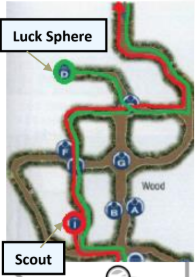
\includegraphics{graphics/kilikamap}}
\begin{enumerate}[resume]
	\item Go left and up the hidden path, \pickup{Scout}. Do not equip, it is sold later.
	\item Teach Tidus Flee via the Sphere Grid
	\item Immediately after crossing the log bridge turn right. Repeatedly run into \textbf{Lord Ochu} and Flee until your encounter count is 159. After the first Flee a crusader will give you 3x Phoenix Down.
\end{enumerate}
\liteversiondetermination{Exclude}{%
\begin{enumerate}[resume]
	\item Continue up the hidden path, following the map, to the temple steps
	\item \sd
	\item \formation{\yuna}{\kimahri}{\lulu}
	\item \save
\end{enumerate}
}
\liteversiondetermination{Include}{%
\begin{enumerate}[resume]
	\item Before Geneaux: \formation{\yuna}{\kimahri}{\lulu}
	\item \save
\end{enumerate}
}
\begin{battle}[3000]{Sinspawn Geneaux}
	\begin{itemize}
		\summon{\valefor}
		\valeforf Fire Tentacle
		\valeforf Fire Tentacle
		\valeforf Fire Main Body x3
		\valeforf Sonic Wings Main Body
		\valeforf Fire Main Body x1-2
	\end{itemize}
\end{battle}
\liteversiondetermination{Exclude}{%
\begin{enumerate}[resume]
	\item \sd\ on stone steps and temple. go into temple. Walk up to \wakka\ and Pray. \sd\ inside temple and go up steps. Wait for lift and \sd.
\end{enumerate}
\begin{trial}
	\begin{itemize}
		\item Take the sphere from the pedestal
		\item Place into the door, take it off of the door.
		\item Place sphere into the next door, take the sphere back.
		\item Place the sphere into the right holder
		\item Touch glpyh
		\item Take the sphere from the next room
		\item Place it into the left holder
		\item Take the glyph sphere from the pedestal
		\item Place it in the Fire Room
		\item Take the sphere that you put into the right holder
		\item Use it to open the door in the Fire Room
		\item Take the sphere off the door
		\item Enter the Fayth room
	\end{itemize}
\end{trial}
\begin{enumerate}[resume]
	\item In Fayth room, \sd, speak to \wakka\ first. Try to leave room, \sd, name \ifrit
	\item Hold down to exit temple, \cs[0:40], \sd
	\item Exit Kilika Woods same way that you entered
	\item Go down and right to S.S. Winno. \sd
\end{enumerate}
}
\liteversiondetermination{Include}{%
\begin{enumerate}[resume]
	\item After the temple exit Kilika Fleeing all encounters
\end{enumerate}
}
	\chapter{S.S. Winno}
\restartlist{enumerate}
\liteversiondetermination{Exclude}{%
\begin{enumerate}
	\item \cs[1:10], exit door on the right. \sd\ with Oaka, then run outside. Go up to the top deck for \wakka\ and \lulu\ cutscene, \sd
	\item Run up to the blitzball on the front of the boat. \cs[1:10]
	\item Follow the tutorial, fail the minigame
	\item \sd\ on \yuna's scene, do not save. \skippablefmv[0:30] if you buffered the Start command in Kilika.
\end{enumerate}
}
\liteversiondetermination{Include}{%
\begin{enumerate}
	\item Don't lend Gil to O'aka here, we will lend to him later.
\end{enumerate}
}
	\chapter{Luca}
\restartlist{enumerate}
\liteversiondetermination{Exclude}{%
\begin{enumerate}
	\item \sd, go right and up to the next screen, \cs[2:30]. Don't save.
	\item \sd\ in locker room. Don't do the tutorial. \sd by mashing another button (like \textbf{R1}) at the same time as confirm, walk down, \sd
	\item Walk down to next screen, \sd. Whistle \cs[0:30], walk right to next screen.
	\item \sd, run to the cafe. \sd, \skippablefmv+\cs[1:20], \sd
	\item Run left to next screen, then left to the docks.
	\item Talk to O'aka.
\end{enumerate}
}
\liteversiondetermination{Include}{%
\begin{enumerate}
	\item Talk to O'aka on the first docks screen, before going into the Machina Fights. Do the following shop:
\end{enumerate}
}
\begin{shop}{10890}
	\begin{itemize}
		\item Sell
		      \begin{itemize}
			      \item All Weapons and Armor, including longsword.
		      \end{itemize}
		\item Buy
		      \begin{itemize}
			      \item Stunning Steel, Equip
		      \end{itemize}
		\item If you have 1100 gil left over, lend O'aka 1100 gil.
	\end{itemize}
\end{shop}
\begin{enumerate}[resume]
	\item Walk up after finishing with O'aka and grab the Chest on the north side of the dock.
	\item Run to the next screen.
\end{enumerate}
\begin{battle}{Machina}
	\begin{itemize}
		\item \textit{For the first two encounters:}
		      \begin{itemize}
			      \tidusf Defend
			      \kimahrif Defend
			      \luluf Thunder
		      \end{itemize}
		\item \textit{For the third encounter:}
		      \begin{itemize}
			      \item \textit{First Wave}
			            \begin{itemize}
				            \tidusf Attack
				            \kimahrif Attack
				            \luluf Thunder a different Machina
				            \tidusf Attack
				            \kimahrif \od\ Seed Cannon \textit{if no crits else} Attack
			            \end{itemize}
			      \item \textit{Second Wave}
			            \begin{itemize}
				            \tidusf Defend
				            \kimahrif Defend
				            \luluf Thunder
			            \end{itemize}
			      \item \textit{Third Wave}
			            \begin{itemize}
				            \tidusf Attack
				            \kimahrif Attack or \od\ Seed Canon
				            \luluf Thunder a different Machina
			            \end{itemize}
		      \end{itemize}
	\end{itemize}
\end{battle}
\liteversiondetermination{Exclude}{%
\begin{enumerate}[resume]
	\item If anyone is Critical HP, use Potions.
	\item Run right. 
\end{enumerate}
}
\begin{battle}[3000]{Oblitzerator}
	\begin{itemize}
		\kimahrif Defend
		\tidusf Defend
		\luluf Thunder Crane x3
		\tidusf Use Crane after 3 Thunders
		\kimahrif Defend
		\luluf Thunder
		\tidusf Attack
	\end{itemize}
	Check for \textbf{Lightning Steel, Thunder Ball}
\end{battle}
\liteversiondetermination{Exclude}{%
\begin{enumerate}[resume]
	\item \cs[2:00], \sd\ during and after Blitzball game.
\end{enumerate}
}
\vfill
\begin{equip}
	\begin{itemize}
		\item \textit{If you got Lightning Steel}
		      \begin{itemize}
			      \tidusf Lightning Steel
		      \end{itemize}
		\item \textit{If you got Thunder Ball}
		      \begin{itemize}
			      \wakkaf Thunder Ball
		      \end{itemize}
	\end{itemize}
\end{equip}
\liteversiondetermination{Exclude}{%
\begin{enumerate}[resume]
	\item Run South for the next two screens. \save. Go up the stairs to the locker room, \sd
	\item Go back into locker room, speak to \wakka, \sd, \cs[1:20]. \sd\ after \lulu\ scene. \cs[1:40] on Auron Entrance.
\end{enumerate}
\vfill
\ 
\columnbreak
\ \newline
\begin{blitzball}
	\begin{itemize}
		\item \textbf{First Half:}
		      \begin{itemize}
			      \item \textit{If Luca wins the Blitzoff:}
			            \begin{itemize}
				            \item Triangle, switch the mode to \textbf{Mark Mode}, and then \textbf{Left Side}
			            \end{itemize}
			      \item \textit{When you get the ball:}
			            \begin{itemize}
				            \item Change to \textbf{Manual A} and \textbf{Normal Mode}
				            \item down some, pass the ball to \tidus
				                  \tidusf Swim next to Jassu, pass to Jassu
				            \item Hide behind the Goalie
				            \item If you aggroed a Goer, Swim Around
			            \end{itemize}
		      \end{itemize}
		\item \sd\ during half time
		\item \textbf{Second Half:}
		      \begin{itemize}
			      \item \textit{If Luca wins the Blitzoff:}
			            \begin{itemize}
				            \item Triangle, switch the mode to \textbf{Mark Mode}, and then \textbf{Right Side}
			            \end{itemize}
			      \item \textit{When you get the ball:}
			      \item Pass to Jassu if he doesn't have it
			      \item Swim to the Bottom Middle
			      \item Wait until 2:20, if Abus Aggros then Break
			      \item Swim to the Left, aggro Balgerda (bottom player), then swim back some
			      \item Pass to \tidus\ before Balgerda gets in range to block
			            \tidusf Swim close to the Goal and Sphere Shot before anyone is close enough to block
			            \begin{itemize}
				            \item If 1 Defender and 2:49, Sphere Shot over the Defender
				            \item Otherwise, Break and Sphere Shot
				            \item If 2 Defenders, Break 1, Sphere Shot
			            \end{itemize}
			      \item \sd\ during \wakka\ \cs
			      \item If you need to Score or it's 1-1, then do the same as above with Jassu
			      \item Wait until 4:20 then aggro Balgerda, Pass to \wakka
			            \wakkaf swim close and Venom Shot, or Break, Venom Shot
		      \end{itemize}
		\item Don't try to score in the First Half
		\item If you're losing, Change to \textbf{Mark Mode} and lose the game.
	\end{itemize}
\end{blitzball}
\begin{enumerate}[resume]
	\item \sd, Don't Save, \cs[1:00]
\end{enumerate}
}
\begin{battle}{Sahagin Chief}
	\begin{itemize}
		\tidusf Attack
		\wakkaf Attack
		\wakkaf Hi-potion anyone who falls below 200 HP
	\end{itemize}
\end{battle}
\liteversiondetermination{Exclude}{%
\begin{enumerate}[resume]
	\item \sd, \skippablefmv
\end{enumerate}
}
\begin{battle}[1800]{Garuda}
	\begin{itemize}
		\tidusf Attack
		\wakkaf Dark Attack
		\auronf Attack
		\wakkaf Attack
		\tidusf Spiral Cut on 3rd turn, if available
		\tidusf Attack
	\end{itemize}
\end{battle}
\liteversiondetermination{Exclude}{%
\begin{enumerate}[resume]
	\item \cs+\skippablefmv[1:30]. Don't save. \sd\ the Auroch scene (PS2 only)
	\item \cs[4:50]. Run north to the hidden chests, \pickup{Magic and HP Sphere}
	\item Run South and try to speak to \auron\ while he's walking away.
	\item Follow red arrow to \yuna. \sd\ during guardian scene. Walk to \yuna, \cs[4:20]
\end{enumerate}
}
\liteversiondetermination{Include}{%
\begin{enumerate}[resume]
	\item \pickup{Magic and HP Sphere}
\end{enumerate}
}
	\chapter{Mi'ihen Highroad}
\restartlist{enumerate}
\textcolor{red}{From this point until the end of Mushroom Rock Road the encounters can be dangerous. Heal after any ambushes and any time Tidus gets hit.}
\liteversiondetermination{Exclude}{%
\begin{enumerate}
	\item Walk up. Forced encounter, \sd. Walk up, \sd\ during Maechen Scene.
\end{enumerate}
}
\begin{encounters}
	\begin{itemize}
		\item Bomb:
		      \begin{itemize}
			      \switch{anyone}{\kimahri}
			      \kimahrif Lancet Bomb, learn \textbf{Self Destruct}
			      \item Flee.
		      \end{itemize}
		\item Else Flee,  Heal afterwards if it was an ambush.
	\end{itemize}
\end{encounters}
\liteversiondetermination{Exclude}{%
\begin{enumerate}[resume]
	\item {Mi'ihen Skip}
	      \begin{itemize}
		      \item After Maechen Scene, run up as quickly as possible.
		      \item Go to the White Spot on the ground towards the left before the Man in Blue
		      \item Speak to the man, get the \textbf{Hunter's Spear}
		      \item Mash and step forward over the cutscene line
		      \item Walk up during the cutscene after the teleport to the next screen.
	      \end{itemize}
	\item Make sure you get the \textbf{Hunter's Spear} if you fail the skip.
	\item Go right and \sd\ at Calli scene. Continue walking up. \sd\ Luzzu scene, \sd\ Shelinda scene
	\item \formation{\tidus}{\wakka}{\auron}
	\item Go to the next screen
	\item Go to the Al-Bhed shop, \sd. Walk out of the shop and \cs[5:30]
	\item Leave shop, \sd. \sd\ on Rin. Walk outside.
\end{enumerate}
}
\liteversiondetermination{Include}{%
\begin{enumerate}[resume]
	\item Get Hunter's Spear
	\item \formation{\tidus}{\wakka}{\auron} before Chocobo Eater
\end{enumerate}
}
\begin{battle}{Chocobo Eater}
	\begin{itemize}
		\item Defend with everyone.
		\item Swap any characters that fall into crit HP with someone in the back.
	\end{itemize}
\end{battle}
\liteversiondetermination{Exclude}{%
\begin{enumerate}[resume]
	\item \sd
	\item Walk north, \save. \important{Lend O'aka 1100 gil if you didn't give it to him earlier.}
	\item Walk north to next screen. Walk to blocked road, \sd. Speak to the guard on the right, \sd, walk back, \sd. Walk up to next screen.
	\item \textit{If you don't have \textbf{Self Destruct}, make sure that you get it before leaving the second screen.}
\end{enumerate}
}
\liteversiondetermination{Include}{%
\begin{enumerate}[resume]
	\item \important{Lend O'aka 1100 gil if you didn't give it to him earlier.}
\end{enumerate}
}
	\chapter{Mushroom Rock Road}
\restartlist{enumerate}
\begin{enumerate}
	\liteversiondetermination{Exclude}{%
	\item \sd, \cs.
	\item Clasko Skip
		\begin{itemize}
			\item Run forward to the 3 Soldiers
			\item Wedge yourself behind the right soldier by holding Left for a second
			\item Tap Down-Right, X to speak to the bottom soldier
			\item If the Soldier got away:
			\begin{itemize}
				\item Run up near the white spot on the wall near the trigger
				\item Talk to the Soldier right after he pushes you into the trigger
				\item Mash until trigger dialogue during the \cs
			\end{itemize}
		\end{itemize}
	}
	\item Flee from all encounters, go to the next screen.
	\item \save. Go up the lift. Follow path.
	\item \formation{\tidus}{\wakka}{\auron}
	\item Early on there is a crusader stood next to a chest, through a rock arch. Open the chest for 1000 Gil
	\item At the end of the first path go up the lift.
	\item Speak to the man immediately ahead of you for an X-Potion
	\item Speak to the man to the left of the next elevator that takes you up to the HQ Elevator, for 400 Gil.
	\item Speak to the man next to the HQ elevator for a Mega-Potion. Go on lift, go to HQ.
	\item Walk down and \sd. Walk right to next screen, then right, \sd. Walk right to O'aka.
	\item Before talking to O'aka:
	\begin{itemize}
		\item Auto-sort Items
		\item \formation{\tidus}{\wakka}{\yuna}
	\end{itemize}
\end{enumerate}
\begin{shop}{10890}
	\begin{itemize}
		\item Sell
			\begin{itemize}
				\item Ethers
				\item X-Potions
				\item Elixirs
				\item Mega-Potions
				\item Hunter's Spear
				\item Any Equipment other than Official Ball, Lightning Steel, Thunder Ball, Stunning Steel
			\end{itemize}
		\item Buy
			\begin{itemize}
				\item Sentry, Equip
			\end{itemize}
	\end{itemize}
\end{shop}
\liteversiondetermination{Exclude}{%
\begin{enumerate}[resume]
	\item \save
	\item \sd, go right, \cs[1:00], \sd\ after Seymour. Go down to guard, use the \nth{2} option to confirm Yes, \sd
\end{enumerate}
}
\vfill\
\end{multicols}
\begin{battle}[12000]{Sinspawn Gui 1}
This fight aims to use Valefor to deal the bulk of the damage with energy blast. After the first energy blast Gui will Attack and follow up with Demi. Then you need to do 3-4 Thunders with Valefor to get Gui to 4218HP or below to kill with Energy Blast. Energy Blast has a damage range of 4218 - 4763 with an average of 4491, so it is possible to kill Gui if its HP is between these values but not guaranteed.
\newline\ \newline
Gui will always follow up an Attack with Demi but can follow up Demi with either an Attack or Demi. Depending on which attacks Gui uses and whether his Attacks miss or not you may only be able to fit in 3 Thunders when a 4th is needed to get Gui below 4218 HP. If Valefor has < 329 HP and Gui just used Demi then Valefor is at risk of dying so you should shield until Gui uses a normal Attack and then use Thunder. After this Thunder use Energy Blast. It is possible that at this point Gui is not dead, however 3 Thunders should be sufficient ~80\%\ of the time.
\newline\ \newline
\textbf{If \yuna\ hit by Thunder:}
	\begin{itemize}
		\tidusf Switch Weapon to Stunning Steel
		\switch{\yuna}{\auron}
		\auronf Power Break Main Body
		\switch{\wakka}{\kimahri}
		\kimahrif Self Destruct main body
		\switch{\tidus}{\yuna}
		\summon{\valefor}
	\end{itemize}
\vspace{\baselineskip}
\textbf{Otherwise:}
	\begin{itemize}
		\switch{\tidus}{\auron}
		\auronf Power Break Main Body
		\yunaf Switch Weapon to Staff
		\switch{\wakka}{\kimahri}
		\kimahrif Self Destruct main body
		\summon{\valefor}
	\end{itemize}
\vspace{\baselineskip}
\textbf{Then:}
	\begin{itemize}
		\valeforf Energy Blast
		\enemyf Attack
		\enemyf Demi
		\valeforf Thunder Body
		\enemyf Attack / Demi
		\valeforf Thunder Body
		\enemyf Attack / Demi
		\valeforf Thunder Body 1x-2x (If HP < 329 and last action was Demi, use shield until gui attacks then use Thunder)
		\valeforf Energy Blast
		\item If Gui still alive: \switch{anyone}{\lulu} and Thunder Gui to death
		\item \textit{If Self Destruct Crit \textit{(3864)}:}
			\begin{itemize}
				\valeforf Energy Blast
				\valeforf Boost
				\valeforf If Gui used demi: Thunder Body
				\valeforf Energy Blast
			\end{itemize}
	\end{itemize}
\end{battle}
\pagebreak
\begin{multicols}{2}
\liteversiondetermination{Exclude}{%
\begin{enumerate}[resume]
	\item \cs+\skippablefmv[2:20]. \sd\ Seymour dialogue.
\end{enumerate}
}
\begin{battle}[6000]{Sinspawn Gui 2}
	\begin{itemize}
		\item \textbf{\textcolor{YellowGreen}{Seymour}}: Thundara Head ($\leftarrow$)
		\item \textbf{\textcolor{YellowGreen}{Seymour}}: Thundara Body x5
		\yunaf Defend
		\auronf Defend
	\end{itemize}
\end{battle}
\liteversiondetermination{Exclude}{%
\begin{enumerate}[resume]
	\item \sd, \cs+\skippablefmv[2:00] (press Start immediately after the skip. Do not use it on the upcoming scenes, as you will crash your game). Walk left and up to Gatta, \sd. \fmv+\cs[1:30], \sd\ during \tidus\ monologue. \cs[1:00], \sd
	\item Walk left, \sd. Walk left, speak to \auron, \sd. \save\ if \auron\ is in critical HP. Go up and right, \sd, exit area, \sd.
\end{enumerate}
%\vfill\ \columnbreak
}


	\chapter{Djose}
\restartlist{enumerate}
\begin{enumerate}
	\item Talk to the guard in Burgundy just to the left and get Soft Ring
	\item \formation{\tidus}{\yuna}{\auron}
	\item Walk North.
\end{enumerate}
\begin{encounters}
	\begin{itemize}
		\item Basilisk:
		      \begin{itemize}
			      \switch{anyone}{\kimahri}
			      \kimahrif Lancet Basilisk, learn \textbf{Stone Breath}
			      \item Flee.
		      \end{itemize}
		\item Else Flee
	\end{itemize}
\end{encounters}
\liteversiondetermination{Exclude}{%
\begin{enumerate}[resume]
	\item Continue walking north, \sd, walk up to the next screen.
	\item Walk along bridge to next screen, \sd, walk into temple. Speak to \auron\ at the doorway, \sd, walk up the stairs.
\end{enumerate}
%\vfill
%\ 
%\columnbreak
%\ \newline
\begin{trial}
	\begin{itemize}
		\item Take the sphere from the left wall
		\item Place into door
		\item Take the sphere from the right wall
		\item Place into door
		\item Take the sphere from the left wall
		\item Push pedestal to the right
		\item Put sphere into the far right wall
		\item Take right sphere
		\item Place into the far right wall
		\item \cs
		\item Take sphere from far right wall
		\item Reset puzzle with the far left tile
		\item Place sphere into pedestal
		\item Take the pedestal sphere
		\item Put sphere into right wall
		\item Take the far right sphere
		\item Put into pedestal
		\item Push pedestal through the door
		\item Jump onto pedestal
		\item Push the second pedestal, return to main room
		\item Take the charged sphere from the right wall
		\item Place charged sphere into the left wall
		\item Reset
		\item Place the two pedestal spheres in the first left and right walls
		\item Go onto the lift in the center
		\item Push all the pedestals in, walk up the stairs
	\end{itemize}
\end{trial}
\begin{enumerate}[resume]
	\item Talk to \auron, wait. \sd, try to leave, \sd, name \ixilon
	\item Speak to \auron, enter the temple and go to the left room. Open the chest for a \textbf{Remedy}. Speak to the priest, \sd. Exit the temple, \sd
	\item Go left, \pickup{4000 Gil}
	\item Cross the bridges, \sd, exit, \sd, go up to Moonflow.
\end{enumerate}
}
\liteversiondetermination{Include}{%
\begin{enumerate}[resume]
	\item Do Auron Affection
	\item Don't need Remedy
	\item Grab 4000 Gil Chest outside temple
\end{enumerate}
}
	\chapter{Moonflow}
\restartlist{enumerate}
\liteversiondetermination{Exclude}{%
	\begin{enumerate}
		\item Walk north, \sd\ on Kimahri Scene.
		\item If \blitzloss: Near the end of the screen, go left through the hidden path. \pickup{Magic Def Sphere}.
		\item Walk north, \sd, walk left, \sd
		\item Talk to O'aka if no Lightning Steel or Thunder Ball
		\begin{shop}{975}
			\begin{itemize}
				\item Buy
					\begin{itemize}
						\item Switch Hitter, Equip
					\end{itemize}
			\end{itemize}
		\end{shop}
		\item walk left past 2 screens, \sd.  Potion/Cure \tidus\ if he got injured. Walk right and use the \nth{2} option to ride ze shoopuf, \sd.
	\end{enumerate}
}
\liteversiondetermination{Include}{%
	\begin{enumerate}
		\item If \blitzloss: \pickup{Magic Def Sphere}.
		\item Talk to O'aka at South Wharf, if no Lightning Steel or Thunder Ball
		\begin{shop}{975}
			\begin{itemize}
				\item Buy
					\begin{itemize}
						\item Switch Hitter, Equip
					\end{itemize}
			\end{itemize}
		\end{shop}
	\end{enumerate}
}
\begin{battle}[4000]{Extractor}
In this fight you need to apply Slow to extractor with Stunning Steel. You can check after each of Tidus' Attacks if Slow has been applied by looking at the turn order. If Slow has been applied Tidus and Wakka will get more than one turn each after some boss turns.
\newline \ \newline
On Extractor's 3rd turn it will rise. After extractor falls back down it will always use Aqua shooter on it's next turn and then it will randomly choose between Aqua Shooter and Rise on subequent turns. You need to deal 500 damage to Extractor once it has risen to force it back down and this is only possible with 4 Attacks, 2 from each of Wakka and Tidus. You need to make sure you always have 4 turns following a turn in which Extractor can rise, so you will need to pay attention to the turn order and use Switch Weapon, where necessary, to fix the turn order to make the fight safe.
\newline \ \newline
	\begin{itemize}
		\tidusf Attack
		\wakkaf Attack
		\tidusf After Slow Applied: Switch Weapon to Lightning Steel/Brotherhood
		\wakkaf Hi-Potion anybody who falls below 250
	\end{itemize}
\end{battle}
\liteversiondetermination{Exclude}{%
\begin{enumerate}[resume]
	\item \sd, walk left to next screen, walk left and talk to \rikku, \sd
	\item Walk up to the forced encounter
\end{enumerate}
}
\begin{battle}{Rikku Tutorial}
	\begin{itemize}
		\item Mash through the tutorial
		\rikkuf Steal from the Treasure Chest
		\rikkuf \od\ Two Potions
		\item Flee
	\end{itemize}
\end{battle}
\begin{enumerate}[resume]
	\item Walk North
	\item \formation{\tidus}{\rikku}{\auron}
	\item Steal from Wolfs / Bees as they have rare steals of Sleeping Powders / Poison Fangs respectively
\end{enumerate}
	\chapter{Guadosalam}
\restartlist{enumerate}
\liteversiondetermination{Exclude}{%
\begin{enumerate}
	\item \sd, walk to Seymour's house, try to leave. Walk into room, speak to \auron, \sd, speak to \wakka, \lulu, \rikku, \yuna. \sd, \skippablefmv+\cs[5:50] if you buffered the Start command after Gui.
	\item Exit the house, walk down, \sd. Go to the Farplane. Hidden to the left in the screen going to the Farplane, \pickup{Lightning Marble x8}
	\item \sd, speak to \auron, go into the Farplane. \cs[1:20]. Speak to \wakka, \sd, speak to \yuna, \cs[2:10], \sd.
	\item Go to Seymour House Entrance, \sd
	\item Guadosalam Skip:
	      \begin{itemize}
		      \item Stand outside of the Potion Shop
		      \item Wait until you get pushed by the Guado to trigger the skip
		      \item Run to the exit using the minimap
		      \item If on HD Remaster, speak to the woman on the left to stop her walking abit, then speak to the running Guado as the woman pushes you to into the door.
	      \end{itemize}
	      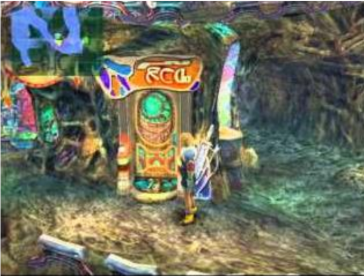
\includegraphics{graphics/guadoskipstandard}

	      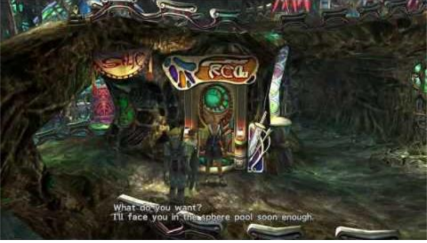
\includegraphics{graphics/guadoskipremaster}
\end{enumerate}
\newpage
}
\liteversiondetermination{Include}{%
\begin{enumerate}
	\item Grab Lightning Marble Chest
\end{enumerate}
}
	\chapter{Thunder Plains}
\restartlist{enumerate}
\begin{enumerate}
	\liteversiondetermination{Exclude}{\item Walk north, dodging lightning.}
	\item Pray (With Square/X) at the cactuar stone just North of the first Lightning Tower
\end{enumerate}
\begin{encounters}
	\begin{itemize}
		\item Steal the following items from Fiends in the Thunder Plains. Always Flee after Stealing.
		\begin{itemize}
			\item Gold Element / Aerouge: 1x Electro Marble
			\item Larva: 2x Lunar Curtain
			\item Qactuar: 1x Chocobo Feather (Can be stolen later in Bikanel if needed. More are better so steal any extras you can.)
			\item Iron Giant: 2x Light Curtain (Only seen in second half of Thunder Plains)
			\item \textbf{(Optional):} Rare steals from lizards for Petrify Grenades, which can be helpful later
		\end{itemize}
		\vspace{\baselineskip}
		\item On the first Iron Giant Fight Defend with \tidus\ and \auron\ so \rikku\ gets hit then Flee
		\vspace{\baselineskip}
		\item On the second Iron Giant Fight, if \yuna\ needs \od:
			\begin{itemize}
				\switch{\rikku}{\yuna}
				\yunaf attack self
				\tidusf defend
				\switch{\auron}{\rikku}
				\rikkuf steal from Iron Giant
				\item Flee
			\end{itemize}
	\end{itemize}
\end{encounters}
\liteversiondetermination{Exclude}{%
\begin{enumerate}[resume]
	\item \sd\ when approaching Al Bhed shop. Walk into the shop when \rikku\ begs to go inside.
\end{enumerate}
}
\begin{shop}{3400}
	\begin{itemize}
		\item Buy:
			\begin{itemize}
				\item 2x Soft
				\item 11x Grenade
			\end{itemize}
	\end{itemize}
	Check to see if you have at least 6313 Gil after the shop
\end{shop}
\liteversiondetermination{Exclude}{%
\begin{enumerate}[resume]
	\item Walk into shop corridor, \cs[2:00]
	\item Speak to \auron, then to \rikku, \sd.
	\item Pickup the \textbf{Yellow Shield} outside the agency if you had less than 6313 Gil after the shop.
	\item Exit screen, go north, near the exit \sd, \cs[3:10]
\end{enumerate}
\vfill
\ 
\colbreak
\ \newline
}
\liteversiondetermination{Include}{%
\begin{enumerate}[resume]
	\item Pickup the \textbf{Yellow Shield} outside the agency if you had less than 6313 Gil after the shop.
\end{enumerate}
}
	\chapter{Macalania Woods}
\restartlist{enumerate}
\begin{enumerate}
	\item \sd, walk north, \sd, \save
	\item \formation{\tidus}{\rikku}{\auron}
	\item Follow path, \pickup{2000 Gil}
	\item Cure \tidus\ if he ever gets damaged.
	\item Make sure that you build up \rikku\ and \yuna\ \od\ before Spherimorph, and that you do the following steals.
\end{enumerate}
\begin{encounters}
	You will need an arctic wind and fish scale for Spherimorph plus up to 2 more Arctic winds and 4 more fish scales later in the run for customising SOS NulFrost and Water Ward respectively. The 2 arctic winds are needed for a backup strategy and the 4 fish scales are optional but helpful. Arctic Winds can also be stolen from Ice Flans in Macalania - Crevasse
	\begin{itemize}
		\item Chimera: Steal Arctic Wind, Flee (Steal up to 3 total)
		\item Blue Elemental: Steal Fish Scale x2, Flee (Steal up to 5 total)
		\item Else: Flee
	\end{itemize}
\end{encounters}
\liteversiondetermination{Exclude}{%
\begin{enumerate}[resume]
	\item Follow path, \sd\ twice
	\item Catch butterfly near the exit to avoid encounters
	\item \formation{\tidus}{\auron}{\kimahri}
	\item \save, talk to Oaka. Say his ``Prices are too expensive'', go in again.
\end{enumerate}
}
\liteversiondetermination{Include}{%
\begin{enumerate}[resume]
	\item \formation{\tidus}{\auron}{\kimahri}
	\item \save, talk to Oaka. Say his ``Prices are too expensive'', go in again.
\end{enumerate}
}
\begin{shop}{9075}
	\begin{itemize}
		\item Sell: Stunning Steel
		\item If less than 9075 Gil, Sell: Yellow Shield
		\item Buy: Sonic Steel, Equip
	\end{itemize}
\end{shop}
\liteversiondetermination{Exclude}{%
\begin{enumerate}[resume]
	\item Run up, \sd. Enter the hidden path, walk to \auron, \sd
\end{enumerate}
}
\begin{battle}[12000]{Spherimorph}
	\begin{itemize}
		\switch{\tidus}{\rikku}
		\rikkuf Grenade, check the Element
		\rikkuf \od, Mag Def Sphere with
		\begin{itemize}
			\item Fire: Arctic Wind
			\item Ice: Bomb Core
			\item Water: Lightning Marble
			\item Thunder: Fish Scale
		\end{itemize}
	\end{itemize}
\end{battle}
\begin{enumerate}[resume]
	\liteversiondetermination{Exclude}{\item \cs[1:50], \sd, \sd}
	\item heal \rikku\ and any other party members who are damaged
	\item \formation{\tidus}{\kimahri}{\auron}
	\item Talk to \auron\ on the way out, then exit
\end{enumerate}

	\chapter{Lake Macalania}
\restartlist{enumerate}
\liteversiondetermination{Exclude}{%
\begin{enumerate}
	\item Run up and \sd
\end{enumerate}
}
\begin{battle}[16000]{Crawler}
	\begin{itemize}
		\switch{\tidus}{\rikku}
		\rikkuf Lightning Marble Crawler
		\rikkuf Lightning Marble Negator		
		\enemyf Gatling Gun
		\kimahrif \textbf{If Negator Survives:} Lancet Negator
		\auronf Phoenix Down \rikku, otherwise Defend
		\rikkuf Lunar Curtain Auron
		\switch{\kimahri}{\tidus}
		\tidusf Phoenix Down \rikku\ / Heal \auron\ / Defend
		\rikkuf Lightning Marble Crawler x2
		\auronf Phoenix Down \rikku\ / Defend
		\auronf \textbf{After Mana Beam:} Phoenix Down Rikku
		\rikkuf \textbf{After 3 Total Lightning Marbles:} Mix Lightning Marble + Lv2. Key Sphere
	\end{itemize}
\end{battle}
\begin{enumerate}[resume]
	\liteversiondetermination{Exclude}{\item \sd, \cs[0:40]}
	\item \important{You need 240 encounters before entering the temple. If you need more encounters you can grind them in the Crevasse. Equip Brotherhood only \textbf{after} grinding encounters.}
\end{enumerate}
\begin{equip}
	\begin{itemize}
		\item Brotherhood
	\end{itemize}
\end{equip}
\liteversiondetermination{Exclude}{%
\begin{enumerate}[resume]
	\item Head to next screen
	\item Head to Temple, \sd. \save, speak to Tromell for \textbf{Shell Targe}
	\item Jyscal Skip:
	      \begin{itemize}
		      \item Walk into the wall to the right of Tromell
		      \item Move slightly to the right, turn around and Talk to Tromell while moving Right.
		      \item If successful, walk forward while mashing Shelinda's dialogue.
		      \item When dialogue finishes, walk up the stairs, push the man, and go through.
		      \item If Shelinda is not saying her dialogue, talk to one of the musicians
	      \end{itemize}
	\item \sd, walk to Fayth room, \cs[2:10]
\end{enumerate}
\vfill\null \columnbreak
}
\begin{battle}[3000]{Seymour}
	\begin{itemize}
		\tidusf Spiral Cut Seymour
		\switch{\yuna}{\rikku}
		\rikkuf Throw Bomb Core / Lightning Marble / Arctic Wind
		\kimahrif Self Destruct Seymour
	\end{itemize}
\end{battle}
\begin{battle}[18000]{Anima}
	\begin{itemize}
		\rikkuf Steal
		\enemyf Pain
		\item \textbf{If \rikku\ survived Pain:}
		\begin{itemize}
			\switch{\rikku}{\yuna}
			\item Grand Summon \shiva
			\shivaf Diamond Dust
			\shivaf Blizarra Anima X2
			\shivaf Blizzara Self
			\shivaf Blizarra Anima x2
		\end{itemize}
		\item \textbf{If \tidus survived Pain:}
		\begin{itemize}
			\switch{\tidus}{\yuna}
			\item Grand Summon \shiva
			\shivaf Blizarra Anima
			\shivaf Diamond Dust
			\shivaf Blizarra Self
			\shivaf Blizarra Anima X3
		\end{itemize}
	\end{itemize}
\end{battle}
\begin{battle}[6000]{Seymour}
	\begin{itemize}
		\shivaf Diamond Dust
	\end{itemize}
\end{battle}
\liteversiondetermination{Exclude}{%
\begin{enumerate}[resume]
	\item Name \shiva
\end{enumerate}
}
\begin{equip}
	\begin{itemize}
		\tidusf Sonic Steel
	\end{itemize}
\end{equip}
\winvfill
\begin{enumerate}[resume]
	\item \formation{\tidus}{\rikku}{\yuna}
\end{enumerate}
\liteversiondetermination{Exclude}{%
\begin{trial}
	\begin{itemize}
		\item \save, exit Fayth room.
		\item Slide pedestal to the right
		\item Take sphere from the right wall, place into pedestal
		\item Push pedestal up
		\item Take Glyph sphere from middle pillar
		\item Go downstairs and push pedestal to the right
		\item Place Glyph sphere in far left slot in the wall
		\item Go upstairs, pick up new sphere
		\item Go downstairs, place sphere in pillar
		\item Go upstairs, take the sphere at the top of the slope
		\item Place in last pillar
	\end{itemize}
\end{trial}
}
\begin{enumerate}[resume]
	\item Go to temple entrance, \sd, Shop with O'aka outside temple
\end{enumerate}
\begin{shop}{17550}
	\begin{itemize}
		\item Buy
			\begin{itemize}
				\item 21x Hi-Potion
				\item 11x Phoenix Down
				\item 2x Antidote
			\end{itemize}
	\end{itemize}
\end{shop}
\begin{enumerate}[resume]
	\item Move south and go down the left path.
	\item Charge Rikku and Yuna Overdrive before Wendigo as follows:
\end{enumerate}
\begin{encounters}
	\begin{itemize}
		\tidusf Escape
		\rikkuf Steal Arctic Wind from Ice Flan if you have less than 2, otherwise steal Sleeping Powders from Wolfs
		\yunaf Attack Self
	\end{itemize}
	Heal after every Battle
\end{encounters}
\begin{enumerate}[resume]
	\item \formation{\tidus}{\yuna}{\lulu}
\end{enumerate}
\begin{battle}[18000]{Wendigo}
	\begin{itemize}
		\switch{\tidus}{\rikku}
		\rikkuf Mix Grenade + Any Purple Sphere
		\yunaf Grand Summon \shiva
		\shivaf Diamond Dust
		\shivaf Blizarra x2-3
	\end{itemize}
\end{battle}
\liteversiondetermination{Exclude}{%
\begin{enumerate}[resume]
	\item Run up to \rikku, \sd, walk up to \yuna, \sd, \save
	\item Don't need any chests under the lake
	\item Run up to \auron\ and speak with him, \sd, walk back, \cs+\skippablefmv[1:00], (press Start immediately after skip), \sd\ in Dream Sequence
\end{enumerate}
}
\liteversiondetermination{Include}{%
\begin{enumerate}[resume]
	\item Don't need any chests under the lake
\end{enumerate}
}
	\chapter{Bikanel Desert}
\restartlist{enumerate}
\liteversiondetermination{Exclude}{%
\begin{enumerate}
	\item Walk up, \sd, walk up
\end{enumerate}
}
\begin{battle}{Zu}
	\begin{itemize}
		\tidusf Attack
		\tidusf Defend
		\enemyf Attack
		\tidusf Defend until \lulu\ shows up
		\auronf Defend until \lulu\ shows up
		\item Flee
	\end{itemize}
\end{battle}
\liteversiondetermination{Exclude}{%
\begin{enumerate}[resume]
	\item \sd
\end{enumerate}
}
\begin{equip}
	\begin{itemize}
		\tidusf Equip Sonic Steel
	\end{itemize}
\end{equip}
\begin{enumerate}[resume]
	\liteversiondetermination{Exclude}{%
		\item Run up to meet with \wakka, \sd. Go left to enter next screen, go right to join with \kimahri, \sd. Run back and then up to meet \rikku, \sd
	}
	\item After \rikku\ cutscene, open chest for 8x Al Bhed Potion
	\item After the Forced Encounter with \rikku: \formation{\tidus}{\wakka}{\auron}
\end{enumerate}
\begin{enumerate}[resume]
	\item Before entering Home you need to achieve the following:
		\begin{itemize}
			\item Fill \rikku\ and \auron\ \od
			\item Steal throwables until you have at least \textbf{15} throwables, including the following:
			\begin{itemize}
				\item 5x Sleeping Powder (Steal from Sand Wolfs)
				\item 2x Smoke Bomb (Steal from Alcyone and Zu)
				\item 2x Silence Grenade (Stolen earlier from Anima)
				\item 2x Shadow Gem (Steal from Sand Worms - Very helpful for Bevelle Guards fights but not strictly necessary)
			\end{itemize}
			\item If you didn't get silence grenades from Anima then steal 2 other throwables in their place
			\item You can steal up to 3 extra throwables, for a total of up to 18, to make some of the later fights faster
		\end{itemize}
	\item Continue along path. On the next screen, go in north-west towards the save sphere, take the shortcut to the left. Go up to the next screen and fight the Sandragora fight at the end of the path, then go up and \sd
\end{enumerate}
\begin{encounters}
	After each encounter reset \formation{\tidus}{\wakka}{\auron}
	\begin{itemize}
		\item Machina x2
			\begin{itemize}
				\tidusf Flee
			\end{itemize}
		\item All other encounters:
			\begin{itemize}
				\switch{\tidus}{\rikku}
				\rikkuf Steal
				\rikkuf Steal again if she survived
				\switch{\wakka}{\tidus}
				\tidusf Flee
			\end{itemize}
	\end{itemize}
\end{encounters}
\begin{enumerate}[resume]
	\item \formation{\tidus}{\wakka}{\rikku}
\end{enumerate}
\begin{battle}{Sandragora}
	\begin{itemize}
		\switch{\tidus}{\auron}
		\auronf \od\ Shooting Star
	\end{itemize}
\end{battle}

\begin{enumerate}[resume]
	\item \formation{\tidus}{\wakka}{\auron}
\end{enumerate}
	\chapter{Home}
\restartlist{enumerate}
\liteversiondetermination{Exclude}{%
\begin{enumerate}
	\item Go into door, \sd
\end{enumerate}
}
\begin{battle}{Bombs}
	\begin{itemize}
		\switch{\tidus}{\rikku}
		\rikkuf Use Silence Grenade (other throwable if no Silence Grenades)
		\rikkuf Use Smoke Bomb
		\auronf Attack Guado twice then defend for rest of fight
		\wakkaf Defend or heal \rikku\ if she gets hit
		\rikkuf Steal from each bomb once
		\rikkuf Throw 2x Grenade or 1x Throwable, if you have any extras
		\item Anyone attack bombs if any remain
	\end{itemize}
\end{battle}
\begin{enumerate}[resume]
	\liteversiondetermination{Exclude}{\item \sd}
	\item \important{Heal Kimahri if he is not full HP}
	\item \formation{\tidus}{\rikku}{\auron} or if you have a Petrify Grenade: \formation{\tidus}{\wakka}{\auron}
\end{enumerate}
\begin{battle}{Dual Horn}
	\begin{itemize}
		\item No Petrify Grenade:
		\begin{itemize}
			\switch{anyone}{\kimahri}
			\kimahrif Lancet Dual Horn
			\kimahrif \od\ Stone Breath
		\end{itemize}
		\item Petrify Grenade:
		\begin{itemize}
			\switch{anyone}{\rikku}
			\rikkuf Use Petrify Grenade
		\end{itemize}
	\end{itemize}
\end{battle}
\begin{enumerate}[resume]
	\item \important{Heal Kimahri if he is not full HP}
	\item \formation{\tidus}{\rikku}{\auron}
	\liteversiondetermination{Exclude}{\item Go down and left, \cs[0:50]}
\end{enumerate}
\begin{battle}{Chimera}
	\begin{itemize}
		\switch{anyone}{\kimahri}
		\kimahrif Lancet Chimera (Aqua Breath)
		\kimahrif \od\ Stone Breath
	\end{itemize}
\end{battle}
%\winvfill
\begin{enumerate}[resume]
	\item Walk down steps, \cs[1:30]
	\item Before going further, \pickup{Level 4 Key Sphere (Chest on left at bottom of stairs)}
	\item Auto Sort Items, Manual Sort Phoenix Downs to top
	\item \formation{\tidus}{\auron}{\kimahri}
	\liteversiondetermination{Exclude}{%
		\item \sd\ until Tidus asks ``why'', \cs[6:20]
		\item Go bottom right to the next screen, run across the bridge
	}
\end{enumerate}
	\chapter{Airship}
\restartlist{enumerate}
\liteversiondetermination{Exclude}{%
\begin{enumerate}
	\item \sd\ during \cs\ +3 \skippablefmv. Walk down corridor to the next screen, go back in, \sd. Speak to Brother, \sd. Walk towards corridor, \sd. Walk towards camera to the next screen, go up and speak to Rin.
	\item \save. Make sure that \rikku\ has \od. If she doesn't, you can get encounters on Rin's first screen.
	\item Shop with rin next to the elevator
\end{enumerate}
}
\liteversiondetermination{Include}{%
\begin{enumerate}
	\item Shop with rin next to the elevator
\end{enumerate}
}
\begin{shop}{6186}
	\begin{itemize}
		\item Sell first 2 weapons / armours in inventory except Soft Ring, Sentry \& Claw
		\item Buy \& Equip:
		\begin{itemize}
			\item Shimmering Blade
			\item Devastator
			\item Seeker's Armlet
			\item Seeker's Bracer
		\end{itemize}
	\end{itemize}
\end{shop}
\newpage
\end{multicols}
\begin{battle}[32000]{Evrae}
	The key to this fight is reducing Evrae's health until it is in the window \textcolor{Red}{[11460-11967]}. Once Evrae is in the damage window you need to perform the killing combo blow but it needs to be well timed. You should try to get Evrae into this window before the second Poison Breath. If you fail to get Evrae into this window before the second Poison Breath it is best to tank another Poison Breath and defend for an extra cycle. Once you are confident with the fight you can judge whether you have the time to get her in the window after the Poison Breath.\newline
	\vspace{\baselineskip}
	\textcolor{Red}{There is a rare outcome where \rikku 's Second Mix crits Evrae (9000+ Damage). Evrae will likely have overshot the damage window and in rare cases Evrae may use haste here. If Evrae hastes then recovery is almost impossible and it is very likely game over. If Evrae is below the damage window do not damage her until next poison breath, Hi-Potion Auron and Phoenix Down Rikku if hit by Evrae.}
	\vspace{\baselineskip}
	\begin{itemize}
		\switch{\tidus}{\rikku}
		\rikkuf Mix Grenade + Purple Sphere
		\kimahrif Hi-Potion \auron\ / Phoenix Down \rikku\ if either gets hit, otherwise spam Attacks
		\auronf Spam Attacks
		\rikkuf Steal x2
		\rikkuf Lunar Curtain \auron
		\rikkuf Use Smoke Bomb / Sleeping Powder (Don't use last Smoke Bomb)
		\rikkuf Use Elemental Damage Item(s)
	\end{itemize}
	\vspace{\baselineskip}
	\begin{itemize}
		\enemyf Poison Breath
	\end{itemize}
	\vspace{\baselineskip}
	\begin{itemize}
		\switch{\auron}{\tidus}
		\tidusf Phoenix Down \rikku
		\tidusf Phoenix Down \kimahri
		\item \textbf{Anyone:} Heal Petrification with Al Bhed Potion / Soft
		\rikkuf Mix Lv.1 Key Sphere + Lv.2 Key Sphere
		\switch{\tidus}{\auron}
		\auronf Antidote Self
		\kimahrif Hi-Potion \auron
		\rikkuf Use Water Gem(s) then 1 Smoke Bomb / Sleeping Powder then elemental damage items
		\item Get Evrae into the damage window here. Once she is in the window defend with all until Poison Breath
	\end{itemize}
	\vspace{\baselineskip}
	\begin{itemize}
		\enemyf Poison Breath
	\end{itemize}
	\vspace{\baselineskip}
	\begin{itemize}
		\switch{\auron}{\tidus}
		\tidusf Phoenix Down \rikku
		\tidusf Phoenix Down \kimahri
		\item \kimahri\ / \tidus\ Heal Petrification with Soft
		\rikkuf Use Smoke Bomb
		\item Killing Combo (Make sure \kimahri\ has a turn between both of \rikku 's turns):
		\begin{itemize}
			\rikkuf Use Smoke Bomb / Sleeping Powder \textcolor{Red}{(If Evrae has already Hasted Skip this step)}
			\kimahrif Self Destruct
			\rikkuf Mix Yellow Sphere + Lv.4 Key Sphere
		\end{itemize}
	\end{itemize}
\end{battle}
\newpage
\begin{multicols}{2}
\liteversiondetermination{Exclude}{%
\begin{enumerate}[resume]
	\item \sd, \skippablefmv[3:00] - Press Start immediately after pressing Square/X.
\end{enumerate}
}
	\chapter{Bevelle}
\restartlist{enumerate}
\begin{enumerate}
	\item Use a Mega-Potion
	\item \formation{\tidus}{\auron}{\kimahri}
\end{enumerate}
\begin{battle}{Guard Fights - Sleeping Powder}
Reset \formation{\tidus}{\auron}{\kimahri} and \textbf{\textcolor{Green}{heal}} after every fight
\vspace{\baselineskip}
	\begin{itemize}
		\item \textbf{Fights 1 and 3:}
			\begin{itemize}
				\switch{\tidus}{\rikku}
				\rikkuf Use Sleeping Powder
				\rikkuf Use 2x Grenade or 1x Throwable if spare
			\end{itemize}
		\item \textbf{Fights 2 and 4:}
			\begin{itemize}
				\item Shadow Gem:
				\begin{itemize}
					\switch{\tidus}{\rikku}
					\rikkuf Sleeping Powder
					\rikkuf Shadow Gem
					\kimahrif Phoenix Down \rikku , otherwise Defend
					\auronf Attack Robot once
					\rikkuf Bomb Core on Robot
					\rikkuf Use Grenade
				\end{itemize}
				\item No Shadow Gem:
				\begin{itemize}
					\switch{\tidus}{\rikku}
					\rikkuf Sleeping Powder
					\rikkuf Bomb Core on Robot
					\kimahrif Phoenix Down \rikku , otherwise Defend
					\auronf Phoenix Down \kimahri, otherwise Attack Robot
					\rikkuf Bomb Core on Robot
					\auronf Attack Robot
					\rikkuf Use Throwable
				\end{itemize}
			\end{itemize}
		\item \textbf{Fight 5:}
			\begin{itemize}
				\switch{\tidus}{\rikku}
				\rikkuf Use Sleeping Powder
				\rikkuf Use Throwable
				\rikkuf Use Bomb Core on Robot
			\end{itemize}
	\end{itemize}
\end{battle}
\liteversiondetermination{Exclude}{%
\begin{enumerate}[resume]
	\item \sd, \skippablefmv[1:30], \sd\ on \yuna\ dialogue. \skippablefmv[30], \sd. Use lift, \sd.
\end{enumerate}
\vfill\ \columnbreak
\begin{trial}
	\begin{itemize}
		\item For all of these you can Hold X instead of pressing it when you get onto the directional pad. The counts of which junction are 1-indexed, starting at the beginning of each area.
		\item Push the pedestal in
		\item Press X
		\item Go left at the second junction
		\item Take sphere, push pedestal back into the junction
		\item At the third junction, go back
		\item Go left at the second junction
		\item Place sphere into wall, push pedestal back
		\item Go left at the first junction
		\item Go left
		\item At the third junction and go right
		\item Take glyph sphere from wall, push pedestal back onto the road
		\item At the fourth junction go right
		\item Place glyph sphere into pedestal
		\item Take Bevelle sphere from pedestal
		\item Place Bevelle sphere into the wall
		\item Take the glyph sphere
		\item Place into the next wall
		\item Take Destruction sphere from the new wall and put it in the pedestal
		\item Take Bevelle sphere from old wall
		\item Push pedestal back and fall off the edge
		\item Go straight
		\item At the third junction go right
		\item Place destruction sphere into wall
		\item Push pedestal back and fall off the edge
		\item Go straight
		\item At the second junction go right
		\item Push pedestal
		\item Go up the stairs, open the chest
	\end{itemize}
\end{trial}
\begin{enumerate}[resume]
	\item \sd, name \bahamut, don't save, \sd
\end{enumerate}
\newpage
}
	\chapter{Via Purifico}
\restartlist{enumerate}
\begin{enumerate}
	\item Run up past the first telepad
	\item Go to the second telepad and travel north.
\end{enumerate}
\begin{equip}
	\begin{itemize}
		\auronf Equip Sentry
		\yunaf If you have 4 Fish Scales, Customise Ring with Water Ward
	\end{itemize}
\end{equip}
\begin{encounters}
	Charge \yuna , \valefor\ and \shiva\ Overdrives as follows:
	\vspace{\baselineskip}
	\begin{itemize}
		\yunaf
		\begin{itemize}
			\item \textbf{If Water Ward:}
				\begin{itemize}
					\yunaf Hi-Potion Self if damaged, otherwise defend
					\auronf Defend Always
					\item Don't revive \auron\ if he dies
					\item Once \yuna\ has her \od\ summon one of the Aeons and charge their \od\
				\end{itemize}
			\item \textbf{Otherwise:}
				\begin{itemize}
					\yunaf Defend
					\auronf Phoenix Down \yuna, or Hi-Potion Self
					\item Once \yuna\ has her \od\ summon one of the Aeons and charge their \od\
				\end{itemize}
		\end{itemize}
		\valeforf
		\begin{itemize}
			\item Sonic Wings x3
			\item If 2 turns in a row: Shield
			\item Boost
			\item Sonic Wings until Maze Larva is below 900 HP (< 750 HP if fewer then 270 Encounters)
			\item Thunder
		\end{itemize}
		\shivaf
		\begin{itemize}
			\item If Shiva ever has 2 turns in a row: Shield
			\item Boost
			\item Blizzard Maze Larva
			\item If fewer than 270 Battles: Heavenly Strike
			\item Blizzara Maze Larva
		\end{itemize}
	\end{itemize}
	\vspace{\baselineskip}
	After Charging All overdrives Finish the remaining fights with Shooting Star
\end{encounters}
\liteversiondetermination{Exclude}{%
\vfill\ \columnbreak
}
\begin{battle}{Isaaru}
	\begin{itemize}
		\item Grothia (8000 HP):
			\begin{itemize}
				\summon{\shiva}
				\shivaf Diamond Dust
			\end{itemize}
		\item Pterya (12000 HP):
			\begin{itemize}
				\yunaf Grand Summon \shiva
				\shivaf Diamond Dust
				\shivaf Boost
				\shivaf Blizzara Pterya
				\shivaf Attack to finish if necessary
			\end{itemize}
		\item Spathi (12000 HP):
			\begin{itemize}
				\summon{\shiva}
				\shivaf Blizzara Spathi x5
				\shivaf Diamond Dust
			\end{itemize}
	\end{itemize}
\end{battle}
\liteversiondetermination{Exclude}{%
\begin{enumerate}[resume]
	\item Swim right and then up
\end{enumerate}
}
\begin{battle}{Evrae Altana}
	\begin{itemize}
		\item Anyone: Phoenix Down/Elixir x2 on Evrae Altana
	\end{itemize}
\end{battle}
\liteversiondetermination{Exclude}{%
\begin{enumerate}[resume]
	\item Swim to exit, \sd
\end{enumerate}
\bothvfill
\bothnp
}
	\chapter{Highbridge}
\restartlist{enumerate}
\begin{enumerate}
	\item \textbf{If you have fewer than 2 Chocobo Feathers:}
		\begin{itemize}
			\item \textbf{Customise and equip:}
				\begin{itemize}
					\item Soft Ring $\rightarrow$ SOS Nulfrost
					\item Targe $\rightarrow$ SOS Nulfrost						
				\end{itemize}
		\end{itemize}
	\item \formation{\tidus}{\yuna}{\rikku}
	\item Walk north
	\item Charge \yuna\ and \rikku\ Overdrive on fights
\end{enumerate}
\begin{encounters}
	\begin{itemize}
		\tidusf Escape
		\rikkuf Attack Self
		\yunaf Attack Self
	\end{itemize}
\end{encounters}
\begin{battle}[36000]{Seymour Natus}
	\begin{itemize}
		\item If 2 or more Chocobo Feathers:
			\begin{itemize}
				\switch{\tidus}{\rikku}
				\rikkuf Use Chocobo Feather on Yuna
				\yunaf Summon \valefor
				\valeforf Energy Blast
				\enemyf Banish Valefor
				\rikkuf Mix Grenade + Purple Sphere
				\yunaf Grand Summon \shiva
				\shivaf Diamond Dust
			\end{itemize}
		\item Otherwise:
			\begin{itemize}
				\switch{\tidus}{\rikku}
				\rikkuf Use Bomb Core / Lightning Marble x2
				\yunaf Hi-Potion Self
				\rikkuf Mix Grenade + Purple Sphere
				\yunaf Defend / Hi-Potion Self if less than 200 HP
				\yunaf After 7 poison ticks on Natus: Summon \valefor
				\valeforf Energy Blast
			\end{itemize}
	\end{itemize}
\end{battle}
\liteversiondetermination{Exclude}{%
\begin{enumerate}[resume]
	\item \sd
	\item Walk to \yuna, \cs+\skippablefmv[10:10]. Walk down, \cs[1:40], walk right, exit Macalania Woods
\end{enumerate}
}
	\chapter{Calm Lands}
\restartlist{enumerate}
\begin{enumerate}
	\item \sd, walk left then at the bottom of ramp run towards the lady sat on the chocobo in the north west Calm Lands
\end{enumerate}
\begin{enumerate}[resume]
	\item \formation{\tidus}{\kimahri}{\auron}
	\item Charge \rikku, \lulu\ and \kimahri\ \od
	\item Steal Poison Fangs from Wasps (need up to 5)
\end{enumerate}
\begin{encounters}
After every fight heal and reset \formation{\tidus}{\kimahri}{\auron}
	\begin{itemize}
		\item If fight contains a Wasp:
		      \begin{itemize}
				\tidusf Escape
				\item Switch whoever survives for \rikku
				\rikkuf Steal from Wasp
		      \end{itemize}
	\end{itemize}
\end{encounters}
\liteversiondetermination{Exclude}{%
\begin{enumerate}[resume]
	\item Talk to the lady on the chocobo and do Wobbly Chocobo training
	\item Get on a chocobo and run back to the south west Calm Lands, up the ramp and to the far right
	\item Interact with the chocobo feather on the ground to jump down
	\item Run into the passageway and on to Remiem Temple
	\item Run across the bridge and to the left hand side of the temple and interact with the sphere on the ground
	\item \sd\ and run to the chocobo on the right hand side of the table
	\item Interact with the chocobo and do the chocobo races. Win with 0 chests and then 3 chests.
	\item Auto-sort items and then manual sort Phoenix Down to slot 2 and Wings to Discovery to slot 1
	\item \formation{\tidus}{\wakka}{\yuna}
	\item Run back to Calm Lands and get on the chocobo then run to Calm Lands exit
\end{enumerate}
}
\liteversiondetermination{Include}{%
\begin{enumerate}[resume]
	\item Talk to the lady on the chocobo and do Wobbly Chocobo training
	\item Go to Remiem Temple
	\item Do Chocobo Races and Win with 0 chests and then 3 chests.
	\item Auto-sort items and then manual sort Phoenix Down to slot 2 and Wings to Discovery to slot 1
	\item \formation{\tidus}{\wakka}{\yuna}
	\item Run back to Calm Lands and get on the chocobo then run to Calm Lands exit
\end{enumerate}
}
\begin{battle}[64000]{Defender X}
	\begin{itemize}
		\tidusf Spiral Cut if available otherwise Attack
		\enemyf Attack
		\switch{anyone}{\lulu}, Swap Weapon
		\switch{anyone}{\rikku}, Mix 2x Wings to Discovery
		\luluf Thunder Fury (7 hits required)
	\end{itemize}
\end{battle}
\liteversiondetermination{Exclude}{%
\begin{enumerate}[resume]
	\item \sd, walk across bridge and up to Mt. Gagazet, \sd
\end{enumerate}
\newpage
}
	\chapter{Mt. Gagazet}
\restartlist{enumerate}
\liteversiondetermination{Exclude}{%
\begin{enumerate}
	\item Walk up, \cs[3:40], walk up, \sd
\end{enumerate}
}
\begin{battle}{Biran and Yenke}
	\begin{itemize}
		\kimahrif Ronso Rage: Aqua Breath
		\kimahrif Lancet Biran then Seed Cannon Biran (Repeat 3x)
		\kimahrif Attack Yenke until defeated
	\end{itemize}
	Pay attention to your drops, need at least 1 Return Sphere but 2 Returns is ideal
\end{battle}
\liteversiondetermination{Exclude}{%
\begin{enumerate}[resume]
	\item The drop from the previous fight will give be one of the following:
		 \begin{itemize}
			 \item 2 Return Spheres
			 \item 1 Return Sphere and 1 Friend Spheres
			 \item 2 Friend Spheres
		 \end{itemize}
 \end{enumerate}
}
\begin{enumerate}[resume]
	\item If you got 2 Friend spheres (\textasciitilde1.5\% chance) then you can't continue. You must reload the autosave and redo the Biran and Yenke Fight to continue.
		\begin{itemize}
			\item Customize:
			\begin{itemize}
				\rikkuf Devastator $\rightarrow$ First Strike
				\luluf \textbf{If 2 Returns:} Moogle $\rightarrow$ First Strike
			\end{itemize}
		\end{itemize}
	\item \formation{\tidus}{\rikku}{\lulu}
\end{enumerate}
\begin{enumerate}[resume]
	\liteversiondetermination{Exclude}{\item Walk up, \sd, \cs[1:20], continue walking up, avoid the gravestones.}
	\item Steal 5x Fire Gems form Bombs
	\item Use Spiral Cut and keep recharging \tidus' \od\ until \tidus\ has learned Slice and Dice
	\item Charge \rikku, \lulu\ and \tidus\ \od\ for Flux fight
\end{enumerate}
\begin{encounters}
	For the remainder of the run, when charging \od\ always do the following 2 things:
	\begin{itemize}
		\item Flee from all ambushes
		\item Always escape with at least one person
	\end{itemize}
\end{encounters}
\begin{enumerate}[resume]
	\item Once you get to Wantz half way along gagazet do the following shop
\end{enumerate}
\begin{shop}{90225}
	\begin{itemize}
		\item Sell 6x Wings to Discovery
		\item Sell Equipment if necessary to get enough Gil (Don't Sell Claw or Shimmering Blade)
		\item Buy \& Equip:
		\begin{itemize}
			\item Haste Targe
		\end{itemize}
	\end{itemize}
\end{shop}
\begin{enumerate}[resume]
	\item Once you're on the Seymour Flux screen, heal everyone except \rikku. \rikku\ must be in critical for this fight
\end{enumerate}
\begin{battle}[70000]{Seymour Flux}
	\begin{itemize}
		\item If you had 2 Return Spheres:
			\begin{itemize}
				\rikkuf Use Silence Grenade if available, otherwise Use Poison Fang
				\tidusf Switch Weapon
				\luluf Switch Weapon
				\rikkuf Mix 2x Wings to Discovery
				\tidusf Slice and Dice
				\luluf Thunder Fury
				\rikkuf Use Fire Gem if Flux Still Alive
			\end{itemize}
		\item If you had 1 Return Sphere (This fight variation has a ~25\% Game Over Chance, if you die reload the autosave):
			\begin{itemize}
				\rikkuf Use Poison Fang
				\tidusf Switch Weapon
				\rikkuf Mix 2x Wings to Discovery
				\tidusf Slice and Dice
				\luluf Thunder Fury
				\rikkuf Use Fire Gem
			\end{itemize}
	\end{itemize}
\end{battle}
\liteversiondetermination{Exclude}{%
\begin{enumerate}[resume]
	\item Walk to the next screen. \skippablefmv[0:20], \sd, walk up to \tidus\ House, go into the center, \sd. Follow the boy outside, speak to him upstairs, \sd.
	\item Walk up to the next screen to enter Gagazet Cave.
\end{enumerate}
}
\begin{equip}
	\begin{itemize}
		\rikkuf Claw
	\end{itemize}
\end{equip}
\begin{enumerate}[resume]
	\item Inside Gagazet cave charge \rikku\ and \tidus\ \od. Behemoth is the best encounter.
	\item Also charge \lulu\ and \yuna\ \od\ if the opportunity presents itself, e.g. a second Behemoth encounter.
	\liteversiondetermination{Exclude}{%
		\item Go up the steps. Go down the left path into the water, \sd, swim up. Go up the steps, play the minigame, return to the previous screen.
		\item Return to Save Sphere, go up and left, then go down the right path, swim up into the next screen. Complete the minigame, \rikku\ Green, \tidus\ Blue, \wakka\ Red. Return.
		\item Go up left path, \sd, continue up the path
	}
\end{enumerate}
\begin{equip}
	\important{Before exiting the cave}
	\begin{itemize}
		\rikkuf Devastator
	\end{itemize}
\end{equip}
\begin{battle}[40000]{Sanctuary Keeper}
	\begin{itemize}
		\rikkuf Mix 2x Wings to Discovery
		\tidusf Slice and Dice
	\end{itemize}
\end{battle}
\begin{enumerate}[resume]
	\liteversiondetermination{Exclude}{\item \sd, \cs[0:50]}
	\item Swap \wakka\ for \lulu\ in party
\end{enumerate}
\begin{equip}
	\begin{itemize}
		\item Equip
		\begin{itemize}
			\auronf Shimmering Blade
		\end{itemize}
		\item Customise
		\begin{itemize}
			\auronf Shimmering Blade $\rightarrow$ First Strike
			\luluf If not already done: Moogle $\rightarrow$ First Strike
		\end{itemize}
	\end{itemize}
\end{equip}
	\chapter{Zanarkand}
\restartlist{enumerate}
\begin{enumerate}
	\liteversiondetermination{Exclude}{%
		\item walk left. \fmv+\cs[2:20]
		\item Move left to the sphere, \sd, \cs[1:40]. Walk further left and follow the path down, \cs[3:20], walk left onto the next screen.
	}
	\item Charge \tidus, \rikku\ and \lulu\ \od. Best Encounters are Behemoth on broken bridge and Defender Z inside the dome.
	\item Also Charge \yuna\ \od\ if not already done.
\end{enumerate}
\begin{enumerate}[resume]
	\liteversiondetermination{Exclude}{\item Continue on the path and into the dome.}
	\item Before Spectral Keeper:
	\begin{itemize}
		\item \formation{\rikku}{\lulu}{\auron}
		\item Heal everyone except \rikku. \important{Rikku must remain in critical HP for the Spectral Keeper fight.}% using the \rikku command raises an error
	\end{itemize}
\end{enumerate}
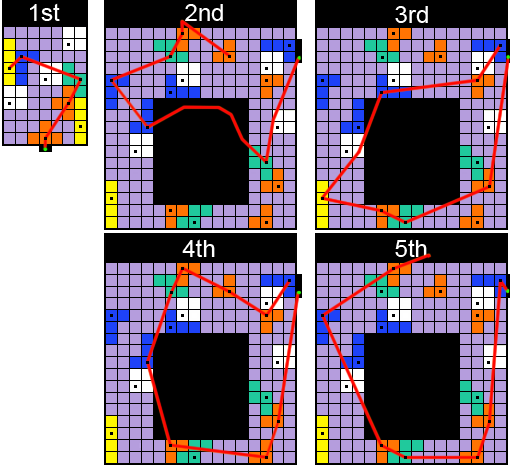
\includegraphics[width=.95\columnwidth]{graphics/Zanarkand_Trials}
\liteversiondetermination{Exclude}{%
\begin{enumerate}[resume]
	\item Push in the pedestals starting from the Top Left, to Bottom Left, then Top Right, Bottom Right, then Besaid Sphere. After pushing in each pedestal, do the corresponding puzzle, shown above.
	\item After the second puzzle, take the Kilika Sphere on the left and put it into the second pedestal.
	\item After the fifth puzzle, take the Besaid Sphere from the right and put it into the fifth pedestal.
	\item \cs, run into the large room
\end{enumerate}
}
\begin{battle}[52000]{Spectral Keeper}
	\begin{itemize}
		\rikkuf Use Light Curtain on \auron
		\auronf Defend
		\luluf Switch Weapon
		\rikkuf Mix 2x Wings to Discovery
		\luluf Thunder Fury (Exactly 5 hits)
		\enemyf Attack All
		\enemyf Berserk Tail
		\auronf Attack
	\end{itemize}
\end{battle}
\begin{enumerate}[resume]
	\item Switch \auron\ for \tidus
	\item If \lulu\ didn't get hit by Spectral Keeper run back out of the Trials and force encounters to charge her \od
	\item Heal everyone except \rikku\ before Yunalesca. \important{Rikku must remain in critical HP for the Yunalesca fight.}% using the \rikku command raises an error
	\liteversiondetermination{Exclude}{\item Run up, \sd\ by mashing another button (like \textbf{R1}) at the same time as confirm, walk up to Yunalesca's room, \sd}
\end{enumerate}
\begin{battle}[132000]{Yunalesca}
	\begin{itemize}
		\rikkuf Light Curtain on Self
		\tidusf Switch Weapon
		\luluf Switch Weapon
		\rikkuf Mix 2x Wings to Discovery
		\switch{\tidus}{\wakka}, Defend
		\switch{\lulu}{\auron}, Hi-Potion \rikku
		\enemyf Dispelling Slap
		\enemyf Absorb
		\wakkaf Hi-Potion \rikku\ if she is damaged, otherwise defend
		\rikkuf Use Fire Gem
		\switch{\auron}{\tidus}, Slice and Dice
		\switch{anyone}{\lulu}, Thunder Fury (7 hits required)
	\end{itemize}
\vspace{\baselineskip}
Check what equipment drops from Yunalesca. Any weapon dropped by Yunalesca will have \textbf{Zombiestrike} which will be important for later.
\end{battle}
\liteversiondetermination{Exclude}{%
\begin{enumerate}[resume]
	\item \sd, leave room, walk down steps, \sd, go down on the next screens, \save, go up the lift, walk out of the cloister of trials, walk down the steps, walk down, \sd\ during \cs+\skippablefmv
\end{enumerate}
}
	\chapter{Airship}
\restartlist{enumerate}
\liteversiondetermination{Exclude}{%
\begin{enumerate}
	\item \sd, walk out of the cockpit past Rin, along the corridors to \yuna\ and \kimahri. \sd. Walk back to the cockpit, \sd. Talk to Cid to travel to Highbridge.
	\item Walk up to the Bevelle entrance, \sd. In the Fayth room, pick the \nth{1} option ``I Think So'', then pick the \nth{2} option ``Defeat Yu Yevon''
	\item Walk up to Cid and search for Omega Ruins (Small Islands just to the right of the mainland)
	\item Travel to Omega Ruins
	\formation{\tidus}{\rikku}{\lulu}
	\item Charge \rikku, \lulu\ and \tidus\ \od
	\item Return to Airship
	\item Switch \tidus\ for \auron
	\item Walk up to Cid, travel to Sin, \sd, \skippablefmv, \sd. Go through the corridors to the outside of the airship, \sd, 3 \skippablefmv[2:10], \sd
\end{enumerate}
}
\liteversiondetermination{Include}{%
\begin{enumerate}
	\item Go to Highbridge
	\item Walk up to Cid and search for Omega Ruins (Small Islands just to the right of the mainland)
	\item Travel to Omega Ruins
	\formation{\tidus}{\rikku}{\lulu}
	\item Charge \rikku, \lulu\ and \tidus\ \od
	\item Return to Airship
	\item Switch \tidus\ for \auron
	\item Walk up to Cid, travel to Sin
\end{enumerate}
}
\begin{battle}[65000]{Sin Left Fin}
	\begin{itemize}
		\rikkuf Mix 2x Wings to Discovery
		\auronf Defend entire fight
		\switch{\lulu}{\kimahri}
		\kimahrif Lancet x7
		\rikkuf Defend until 6th Lancet then Switch Weapon until sin swipes
		\enemyf Sin Swipes
		\switch{\auron}{\lulu}, Thunder Fury
		\luluf Spam Thunder to finish if needed
	\end{itemize}
\end{battle}
\liteversiondetermination{Exclude}{%
\begin{enumerate}[resume]
	\item \sd, \cs+\skippablefmv
\end{enumerate}
}
\begin{battle}[65000]{Sin Right Fin}
	\begin{itemize}
		\rikkuf Mix 2x Wings to Discovery
		\switch{\lulu}{\auron}
		\auronf Defend entire fight
		\rikkuf Use Al-Bhed Potion
		\kimahrif Lancet x5
		\rikkuf Defend until 4th Lancet then Switch Weapon until sin swipes
		\enemyf Sin Swipes
		\switch{\auron}{\lulu}, Spam Thunder to finish
	\end{itemize}
\end{battle}
\liteversiondetermination{Exclude}{%
\begin{enumerate}[resume]
	\item \sd, \cs+\skippablefmv
\end{enumerate}
}
\begin{battle}[56000]{Sin Genais and Core}
	\begin{itemize}
		\switch{\rikku}{\tidus}, Switch Weapon
		\switch{\lulu}{\rikku}, Mix 2x Wings to Discovery
		\tidusf Slice and Dice
		\rikkuf Use Fire Gem
	\end{itemize}
	Check to see if the first equipment drop listed is a weapon. If it is it will have \textbf{Zombiestrike}.
\end{battle}
\liteversiondetermination{Exclude}{%
\begin{enumerate}[resume]
	\item \sd, \skippablefmv
	\item Walk along the corridors to the outside of the ship, speak to \yuna. \cs[1:40], \sd\ \rikku\ dialogue. \skippablefmv.
	\item Walk back into the cockpit area and talk to Cid. Travel to Omega Ruins.
	\formation{\tidus}{\rikku}{\lulu}
	\item Charge \rikku\ and \lulu\ \od
	\item Return to Airship
	\item If no Zombiestrike weapon dropped from Yunalesca or Sinspawn Genais:
	\begin{itemize}
		\item Talk to Rin in the corridor and buy 70x Holy Water
		\item Customise Claw $\rightarrow$ Zombietouch
		\item Customse Staff $\rightarrow$ First Strike
	\end{itemize}
	\item Otherwise:
	\begin{itemize}
		\item Equip Zombiestrike Weapon
		\item Customise Staff $\rightarrow$ First Strike
		\item Customise Zombiestrike Weapon $\rightarrow$ First Strike
	\end{itemize}
	\item Switch \tidus\ for \kimahri\ in party
	\item Go through the corridors, go outside again, \skippablefmv, \sd.
\end{enumerate}
}
\liteversiondetermination{Include}{%
\begin{enumerate}[resume]
	\item \yuna\ cutscene outside
	\item Walk back into the cockpit area and talk to Cid. Travel to Omega Ruins.
	\formation{\tidus}{\rikku}{\lulu}
	\item Charge \rikku\ and \lulu\ \od
	\item Return to Airship
	\item If no Zombiestrike weapon dropped from Yunalesca or Sinspawn Genais:
	\begin{itemize}
		\item Talk to Rin in the corridor and buy 70x Holy Water
		\item Customise Claw $\rightarrow$ Zombietouch
		\item Customse Staff $\rightarrow$ First Strike
	\end{itemize}
	\item Otherwise:
	\begin{itemize}
		\item Equip Zombiestrike Weapon
		\item Customise Staff $\rightarrow$ First Strike
		\item Customise Zombiestrike Weapon $\rightarrow$ First Strike
	\end{itemize}
	\item Switch \tidus\ for \kimahri\ in party
\end{enumerate}
}
\begin{battle}[140000]{Overdrive Sin}
	\begin{itemize}
		\rikkuf Mix 2x Wings to Discovery
		\luluf Thunder Fury
		\kimahrif Lancet
		\rikkuf Use Gem
		\item Finish with Thunder / Lancet / Attacks if needed
	\end{itemize}
\end{battle}
\liteversiondetermination{Exclude}{%
\begin{enumerate}[resume]
	\item \skippablefmv[1:20], \sd
\end{enumerate}
}
	\chapter{Inside Sin}
\restartlist{enumerate}
\begin{enumerate}
	\item \formation{\tidus}{\lulu}{\rikku}
	\item Walk along the path
	\item Charge \tidus, \lulu\ and \rikku\ \od
	\item Charge \yuna\ \od\ if you haven't done it yet
	\liteversiondetermination{Exclude}{%
		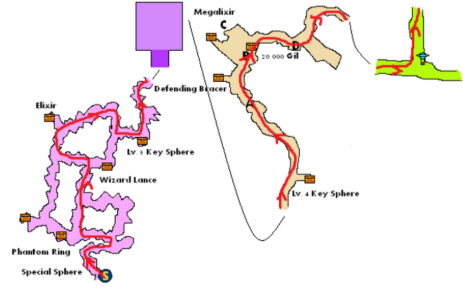
\includegraphics{graphics/sinpath}
		\item Go up the steps, \sd
	}
\end{enumerate}
\begin{battle}[80000]{Seymour Omnis}
	\begin{itemize}
		\rikkuf Mix 2x Wings to Discovery
		\tidusf Slice and Dice (Intentionally Fail)
		\luluf Thunder Fury (6 hits required)
	\end{itemize}
\end{battle}
\begin{enumerate}[resume]
	\liteversiondetermination{Exclude}{\item \sd, walk north.}
	\item Charge \tidus, \lulu\ and \rikku\ \od
	\item Charge \yuna\ \od\ if you haven't done it yet
	\liteversiondetermination{Exclude}{\item Turn left onto the bridge, go onto the next screen.}
	\item Heal everyone except \rikku. \important{Rikku must remain in critical HP for the BFA fight.}% using the \rikku command raises an error
	\liteversiondetermination{Exclude}{\item Complete the minigame, picking up the eggs and avoiding the crystals.}
\end{enumerate}
\liteversiondetermination{Exclude}{%
\begin{enumerate}[resume]
	\item Walk up to Jecht, \cs[4:30]
\end{enumerate}
}
\vfill\ \colbreak
\begin{battle}[180000]{Braska's Final Aeon}
	\begin{itemize}
		\tidusf Talk
		\switch{\yuna}{\rikku}, Use Chocobo Feather on \tidus
		\switch{\auron}{\yuna}, Switch Weapon
		\rikkuf Switch Weapon
		\switch{\yuna}{\lulu}, Switch Weapon
		\rikkuf Mix 2x Wings to Discovery
		\tidusf Talk
		\switch{\lulu}{\kimahri}, Lancet
		\tidusf Slice and Dice
		
		\vspace{\baselineskip}

		\switch{\rikku}{\yuna}, Grand Summon Shiva
		\shivaf Diamond Dust
		\switch{\kimahri}{\rikku}, Use Fire Gem
		\switch{\tidus}{\lulu}, Thunder Fury (7 Hits Required)
	\end{itemize}
\end{battle}
\colend
\liteversiondetermination{Exclude}{%
\begin{enumerate}[resume]
	\item \cs+\skippablefmv[4:00]
\end{enumerate}
}
\begin{battle}{Possessed  Aeons}
	In the Aeon fights you need up to 4 poison fangs. If you have 2 or fewer Poison Fangs prioritise using them on Ifrit and Ixion.
	\begin{itemize}
		\valeforf Throw Poison Fang (or 2x Bomb Core / Lightning Marble / Arctic Wind / Dream Powder if short on Poison Fangs)
		\ifritf Throw Poison Fang + any non-fire throwable
		\ixionf Throw Poison Fang + any non-lightning throwable
		\shivaf Throw Poison Fang (or 2x Bomb Core / Lightning Marble / Arctic Wind / Dream Powder if short on Poison Fangs)
		\bahamutf
			\begin{itemize}
				\rikkuf Throw Bomb Core / Lightning Marble / Arctic Wind / Dream Powder
				\switch{\yuna}{\kimahri}
				\kimahrif Self Destruct
			\end{itemize}
	\end{itemize}
\end{battle}
\liteversiondetermination{Exclude}{%
\begin{enumerate}[resume]
	\item \cs[1:40]
\end{enumerate}
}
\begin{battle}[99999]{Yu Yevon}
	\begin{itemize}
		\item \rikku\ Zombiestrike Weapon:
			\begin{itemize}
				\rikkuf Attack
				\item Anyone Throw Phoenix Down at Yu Yevon
			\end{itemize}
		\item \lulu\ Zombiestrike Weapon:
			\begin{itemize}
				\rikkuf Switch Weapon
				\luluf Attack
				\rikkuf Throw Phoenix Down at Yu Yevon
			\end{itemize}
		\item \kimahri\ Zombiestrike Weapon:
			\begin{itemize}
				\rikkuf Switch Weapon
				\kimahrif Attack
				\item Anyone Throw Phoenix Down at Yu Yevon
			\end{itemize}
		\item Anyone Else Zombiestrike Weapon:
			\begin{itemize}
				\switch{\rikku}{character with Zombie Strike Weapon}
				\item That Character: Attack
				\item Anyone Throw Phoenix Down at Yu Yevon
			\end{itemize}
		\item \rikku\ Zombietouch Weapon:
			\begin{itemize}
				\rikkuf Switch Weapon to Zombietouch Weapon
				\luluf Switch Weapon
				\rikkuf Attack
				\luluf If Curaga deals 9999 damage to Yu Yevon (White numbers) Throw Phoenix Down at Yu Yevon, otherwise Switch Weapon
				\item Keep switching weapon on \lulu\ and \kimahri\ until \rikku\ lands Zombie status and the curaga numbers are white
				\item Once curaga lands, anyone Throw Phoenix Down at Yu Yevon
			\end{itemize}
	\end{itemize}
\end{battle}
\bothvfill
\colstart
\end{multicols}

\end{document}